%%% TeX-command-extra-options: "-shell-escape"
%!TEX options=--shell-escape

%----------------------------------------------------------------------------------------
%   PACKAGES AND THEMES
%----------------------------------------------------------------------------------------
\documentclass[aspectratio=169,xcolor=dvipsnames]{beamer}
% \usetheme{Simple}

\usepackage{pgfpages}

%\setbeameroption{show notes}
\setbeameroption{show notes on second screen}
\setbeamertemplate{note page}[plain]

\usepackage{hyperref}
\usepackage{graphicx} % Allows including images
\usepackage{booktabs} % Allows the use of \toprule, \midrule and \bottomrule in tables
\usepackage{nicefrac}

% hyperlinks
\usepackage{hyperref}
\hypersetup{
    colorlinks=true,
    linkcolor=, % no color for internal links
    filecolor=magenta,
    urlcolor=blue,
}

% code
% \usepackage{minted}
% \setminted{
%     fontsize=\footnotesize,
%     autogobble,
%     bgcolor=mygray,
%     fontsize=\small
% }

% colors
\usepackage{xcolor}
\definecolor{mygray}{gray}{0.95} % define color - grey scale: 0=dark - 1=light

% packages added with respect to overleaf
\usepackage[utf8]{inputenc}
\usepackage{lmodern}
\usepackage{textcomp}
\usepackage[most]{tcolorbox} % colored boxes

% custom commands
\definecolor{darkred}{HTML}{CC0000}
\newcommand\textveryimp[1]{\textcolor{darkred}{\underline{\textbf{#1}}}} % text bold+red+underlined
\newcommand\textimp[1]{\underline{\textbf{#1}}} % text bold+red+underlined
\newcommand\textcode[1]{\textcolor{gray}{\texttt{#1}}} % text typewriter font + gray

\newcommand\blfootnote[1]{%
  \begingroup
  \renewcommand\thefootnote{}\footnote{#1}%
  \addtocounter{footnote}{-1}%
  \endgroup
}

% figures
\usepackage{tikz}
% \usetikzlibrary{shapes,backgrounds}
\usepackage{animate}
%\usepackage{media9}
% equations
\usepackage{amsmath}
\usepackage{amssymb}
\usepackage{empheq}
\usepackage{makecell}

% images
\graphicspath{ {./images/} } % Relative path to image directory

% insert table of content before each section
% \AtBeginSection[]
% {
%     \begin{frame}
%         \frametitle{Table of Contents}
%         % \tableofcontents[currentsection]
%     \end{frame}
% }
% \setbeamertemplate{subsection in toc}[subsections numbered] % add numbers in front of subsections
% \setbeamertemplate{subsection in toc}{\leavevmode\leftskip=2em$\bullet$\hskip1em\inserttocsubsection\par} % add bullets in front of subsections
%\setbeamertemplate{subsection in toc}{\leavevmode\leftskip=3.2em\rlap{\hskip-2em\inserttocsectionnumber.\inserttocsubsectionnumber}\inserttocsubsection\par}
\setbeamertemplate{subsection in toc}{\leavevmode\leftskip=3.5em\rlap{\hskip-1.25em\inserttocsubsectionnumber.}\inserttocsubsection\par} % add indented subsection number

\setbeamerfont{frametitle}{size=\scriptsize} % Set slide title fontsize
\setbeamercovered{transparent} % Set text to be semi-transparent during sequential overlay


%----------------------------------------------------------------------------------------
%   TITLE PAGE
%----------------------------------------------------------------------------------------

\title[short title]{Convolutional Neural Networks II}
\subtitle{Lecture 11}
\author{Automatic Image Analysis}
\titlegraphic{
  
\includegraphics[height=3cm]{cvlogo}
  
\includegraphics[height=3cm]{tublogo}
}
%\date{2021-04-23}

%----------------------------------------------------------------------------------------
%   PRESENTATION SLIDES
%----------------------------------------------------------------------------------------

\begin{document}

\begin{frame}
    \titlepage
\end{frame}


%\begin{frame}{Winners ImageNet Large Scale Visual Recognition Challenge}
  \begin{figure}
    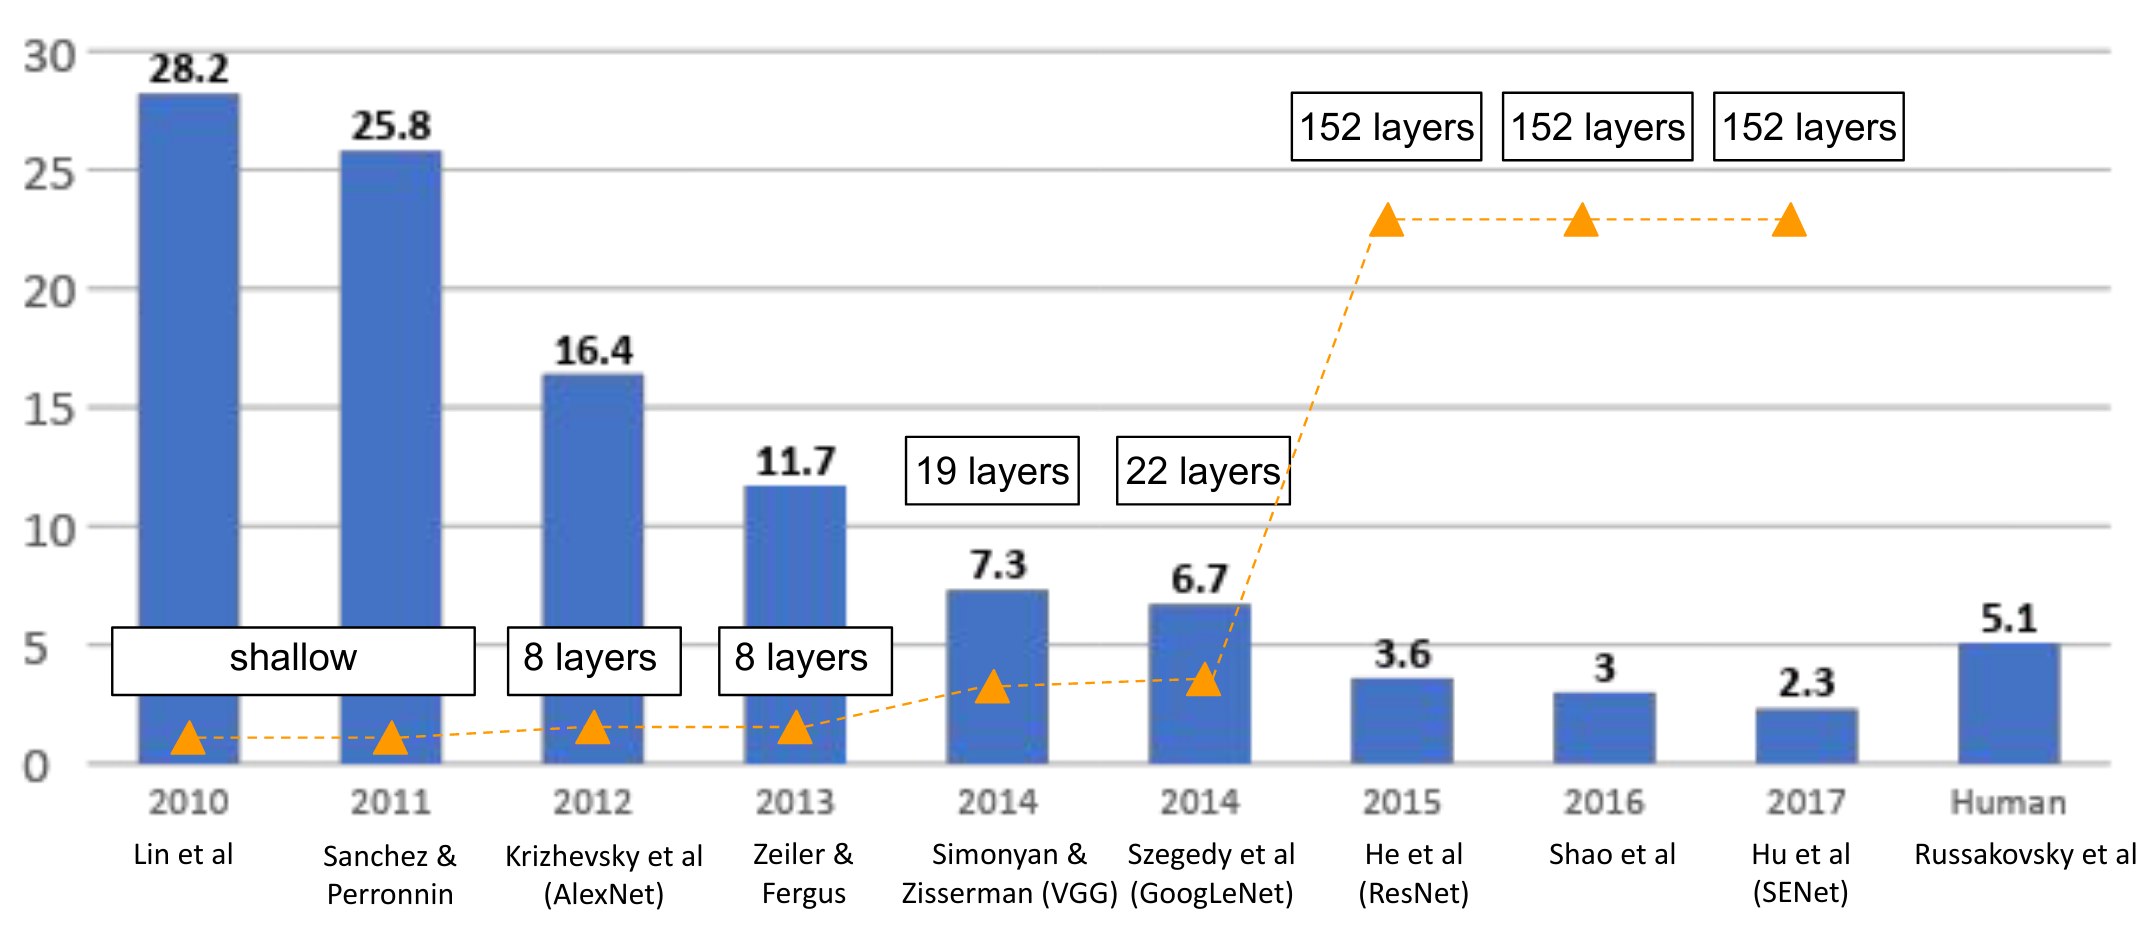
\includegraphics[width=0.9\textwidth]{winners}
  \end{figure}

  \note{
    \begin{itemize}
      \item Image from Stanford CS231n Lecture 9, Fei-Fei Li \url{http://cs231n.stanford.edu/slides/2021/lecture_9.pdf}
    \end{itemize}
  }
\end{frame}


\begin{frame}{Accuracy ImageNet Ops/Params}
  \begin{figure}
    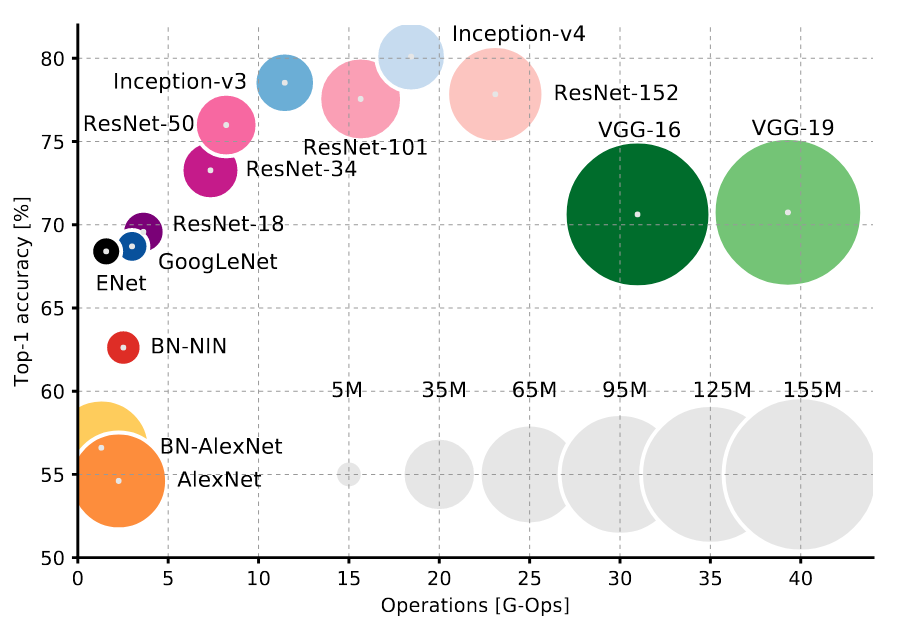
\includegraphics[width=0.7\textwidth]{accuracy_imagenet_params_flops}
  \end{figure}

  \note{
    \begin{itemize}
      \item Image from An Analysis of Deep Neural Network Models for Practical Applications, Canziani et al, 2017
    \end{itemize}
  }
\end{frame}


\begin{frame}{Efficiency}
  \begin{figure}
    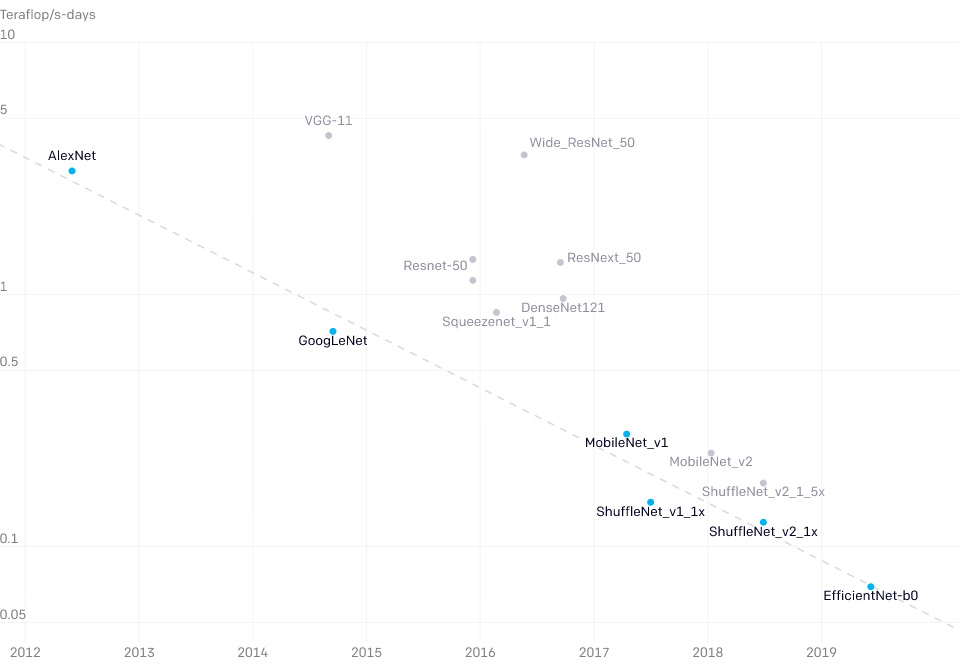
\includegraphics[width=0.8\textwidth]{efficiency}
  \end{figure}

  \note{
    \begin{itemize}
      \item Total amount of compute in teraflops/s-days used to train to AlexNet level performance. Lowest compute points at any given time shown in blue, all points measured shown in gray.
      \item Image from \url{https://openai.com/blog/ai-and-efficiency/}
    \end{itemize}
  }
\end{frame}

\begin{frame}{Semantic Segmentation}
  \begin{figure}
    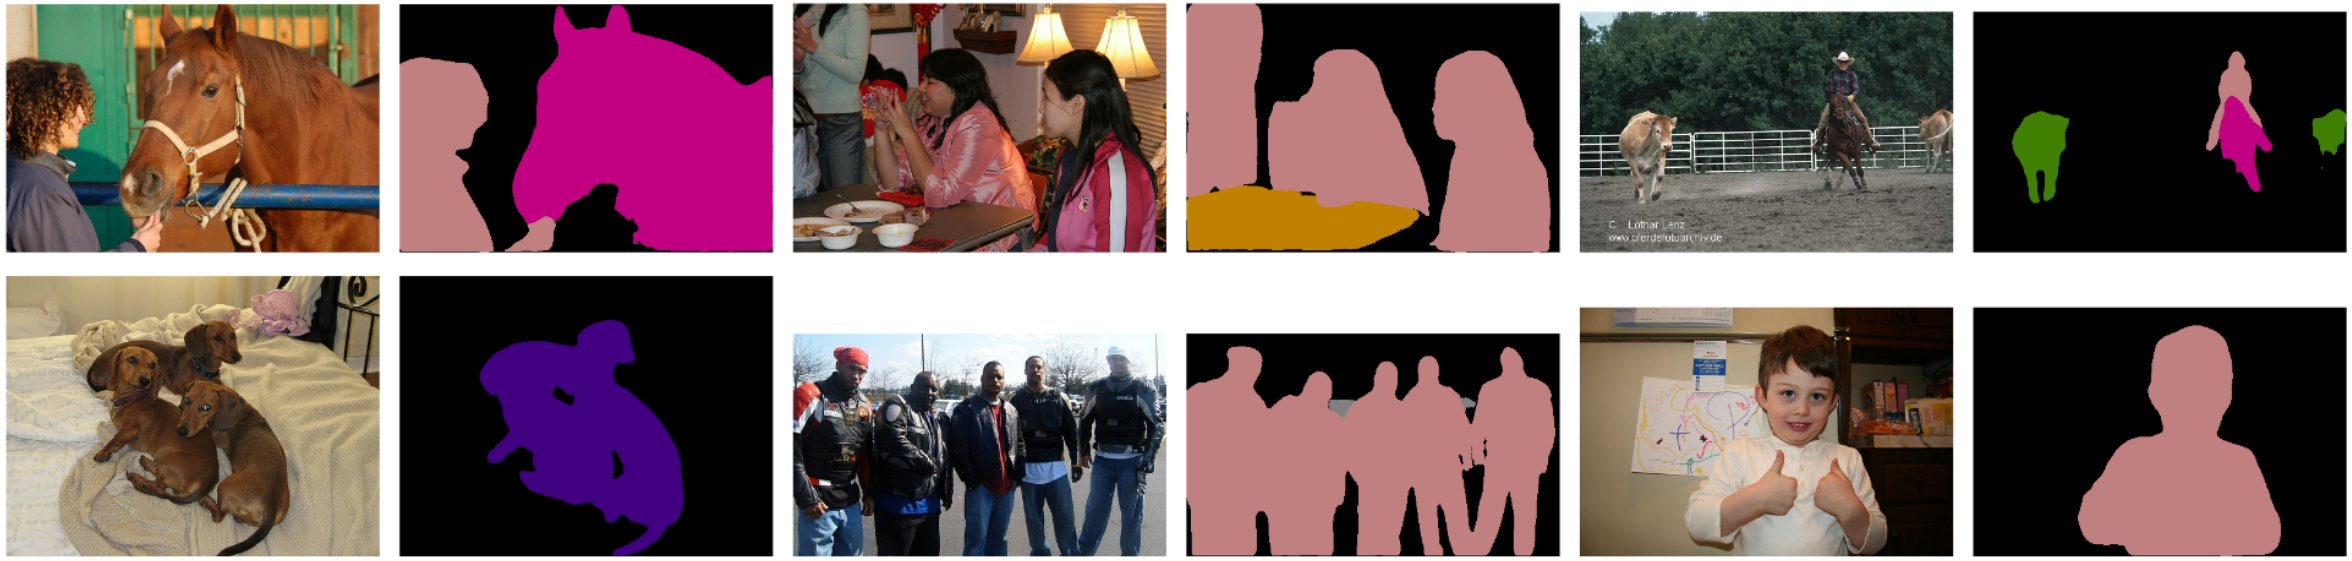
\includegraphics[width=0.9\textwidth]{deeplabv3p_result_00}
  \end{figure}
  \note{
    \begin{itemize}
      \item Semantic Segmentation is the task of classifying every pixel of an image with an object class.
      \item Often including a background class.
    \end{itemize}
  }
\end{frame}


\begin{frame}{Dataset: Cityscapes}
  \begin{columns}
    \begin{column}{0.48\textwidth}
      \begin{figure}
        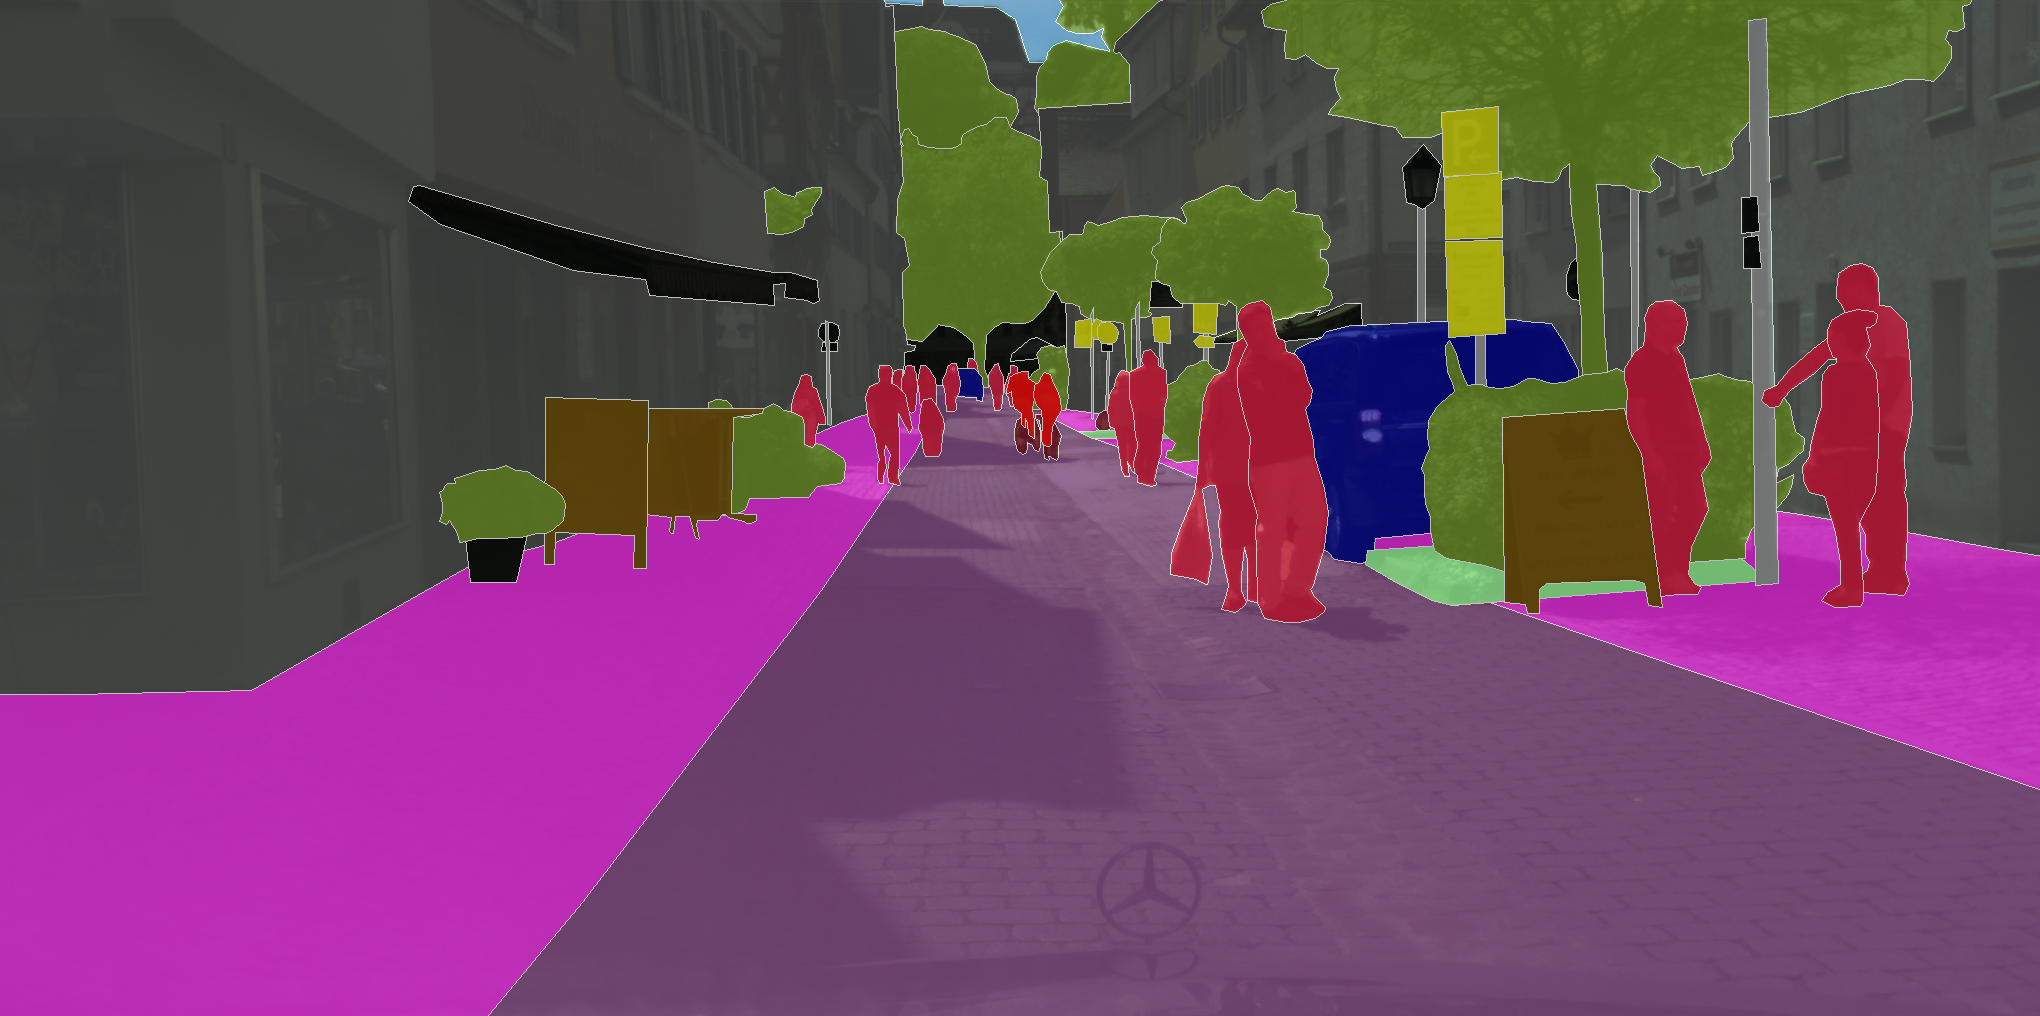
\includegraphics[width=0.9\textwidth]{segmentation_cityscape_tuebingen}
      \end{figure}
    \end{column}
    \begin{column}{0.48\textwidth}
    \begin{itemize}
      \item 30 classes
      \item 5000 annotated images with fine annotation
      \item 20000 annotated images with coarse annotations
    \end{itemize}

    \end{column}
  \end{columns}

\end{frame}


\begin{frame}{Dataset: COCO Common Objects in Context }
  \begin{columns}
    \begin{column}{0.48\textwidth}
      \begin{figure}
        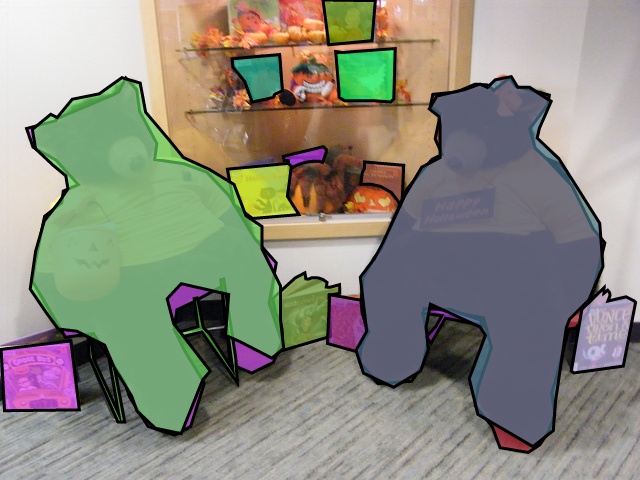
\includegraphics[width=0.9\textwidth]{segmentation_coco_bears}
      \end{figure}
    \end{column}
    \begin{column}{0.48\textwidth}
    \begin{itemize}
      \item 1.5 million object instances
      \item 80 object categories
      \item 91 stuff categories
      \item 330K images ($>$200K labeled)
    \end{itemize}

    \end{column}
  \end{columns}

\end{frame}



\begin{frame}{Semantic Segmentation: sliding window?}
  \begin{figure}
    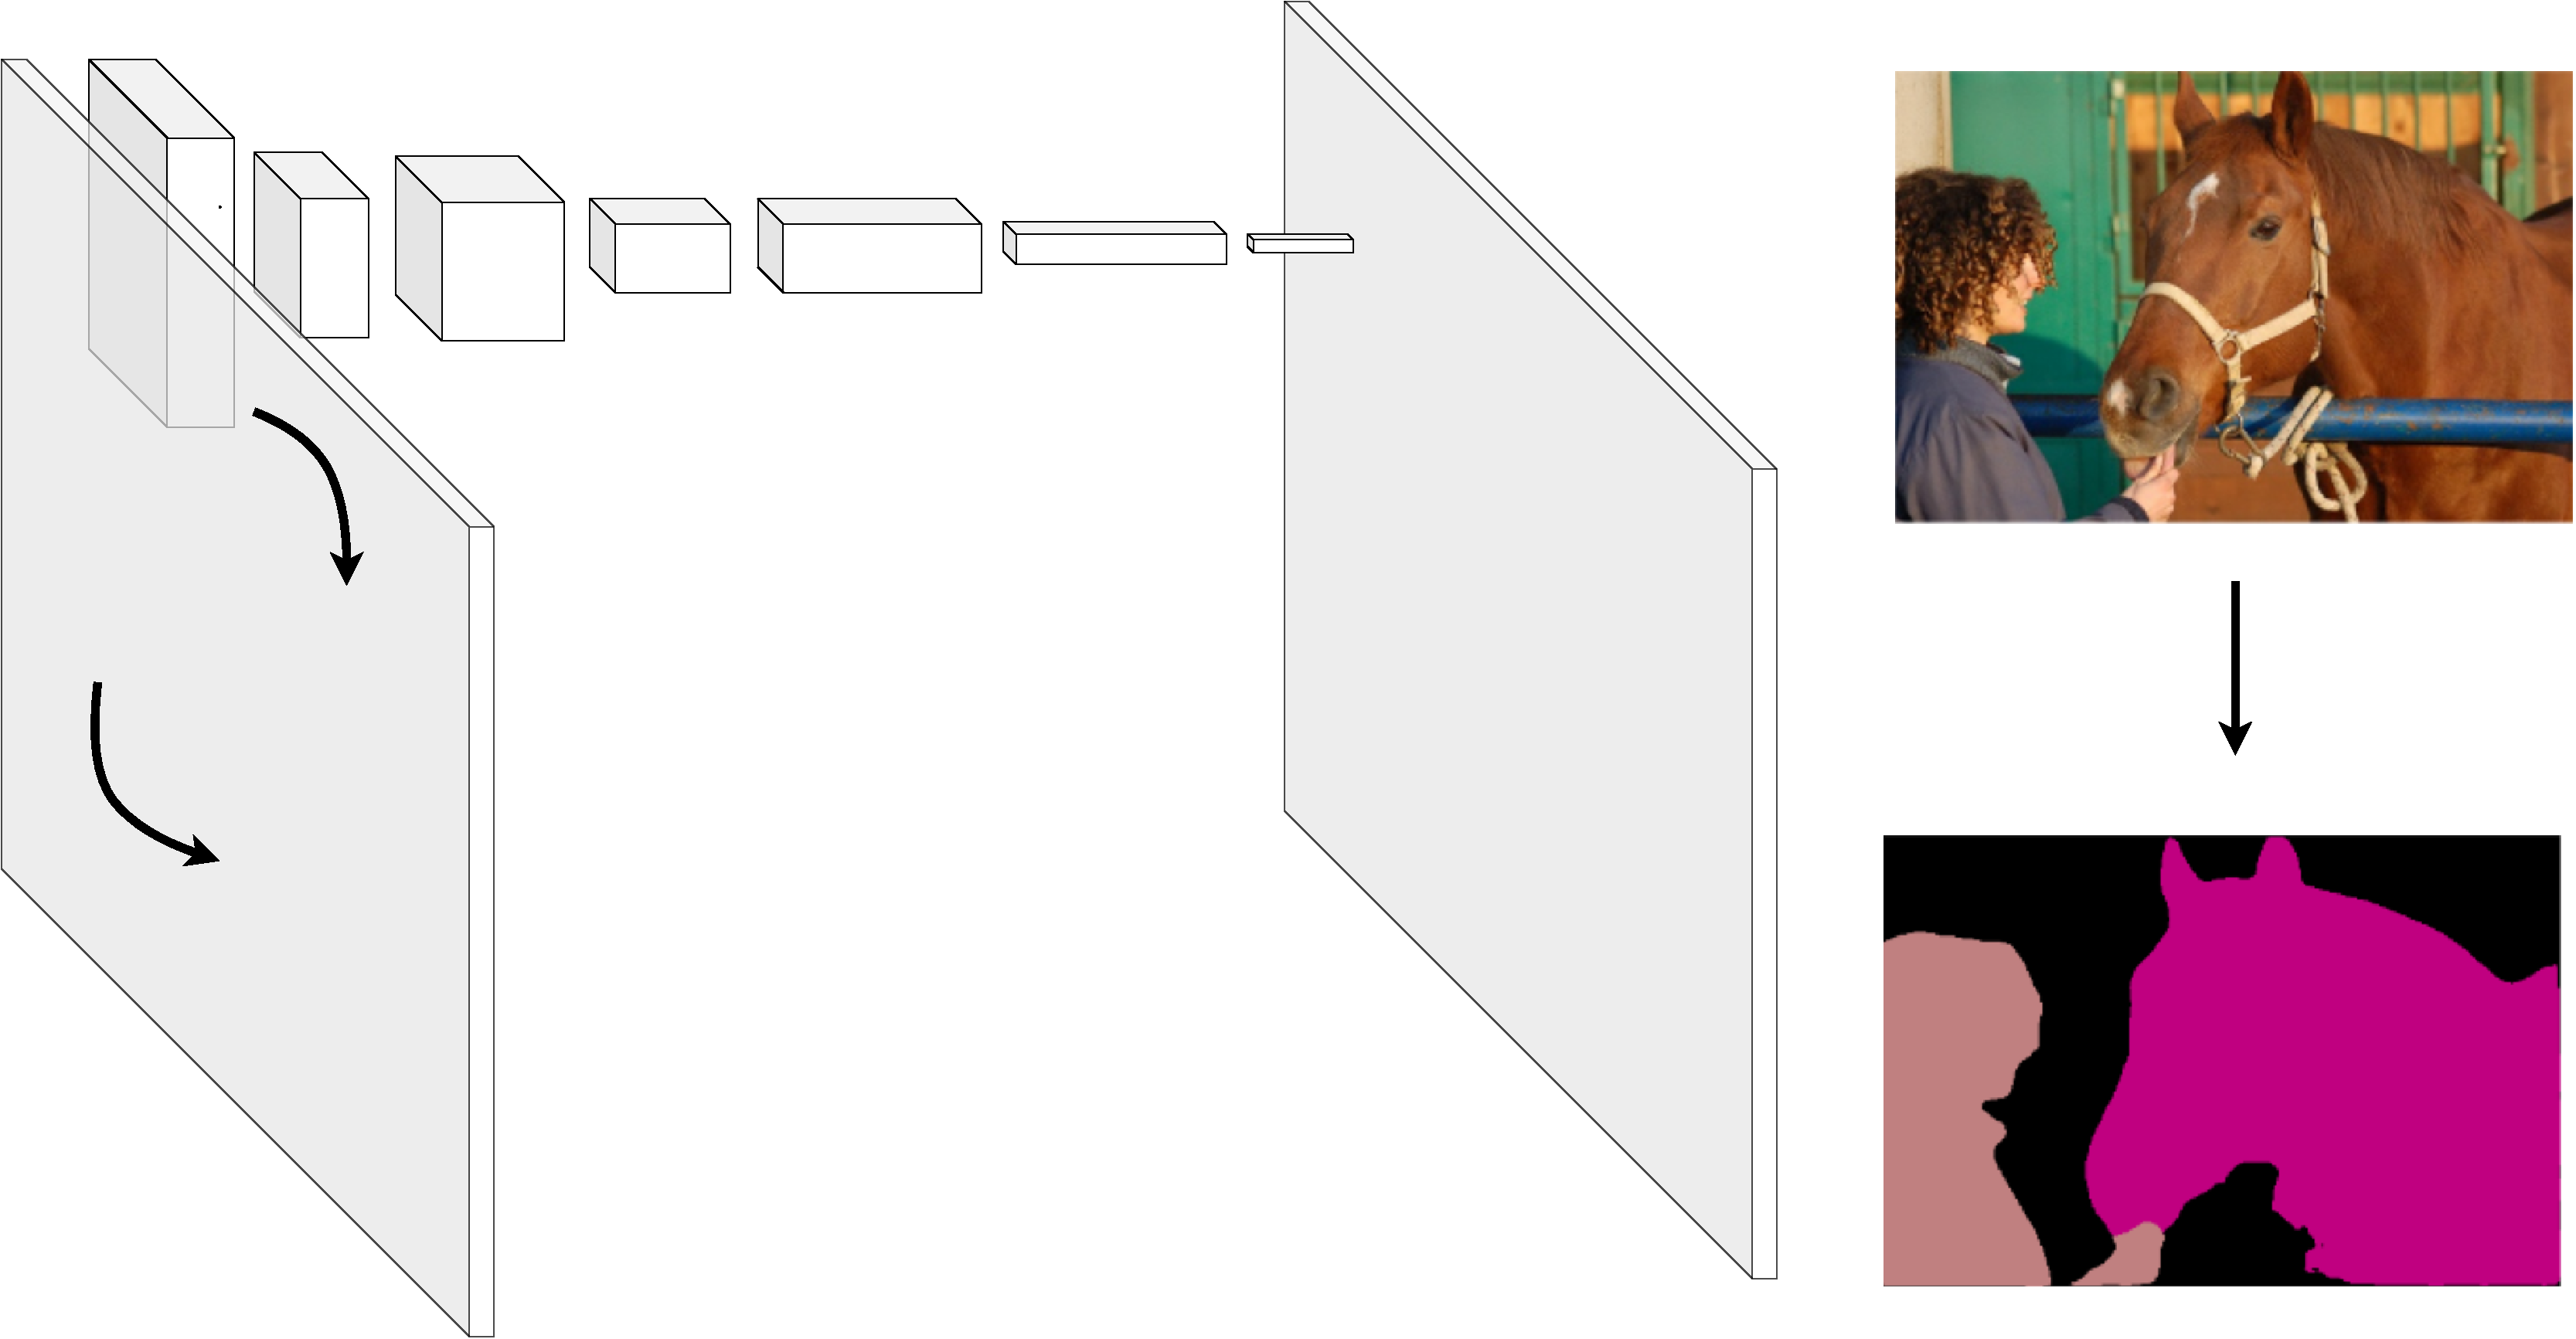
\includegraphics[width=0.9\textwidth]{segmentation_sliding_window}
  \end{figure}

  \note{
    \begin{itemize}
      \item One forward pass per pixel.
    \end{itemize}
  }
\end{frame}


\begin{frame}{Semantic Segmentation: without downsampling?}
  \begin{figure}
    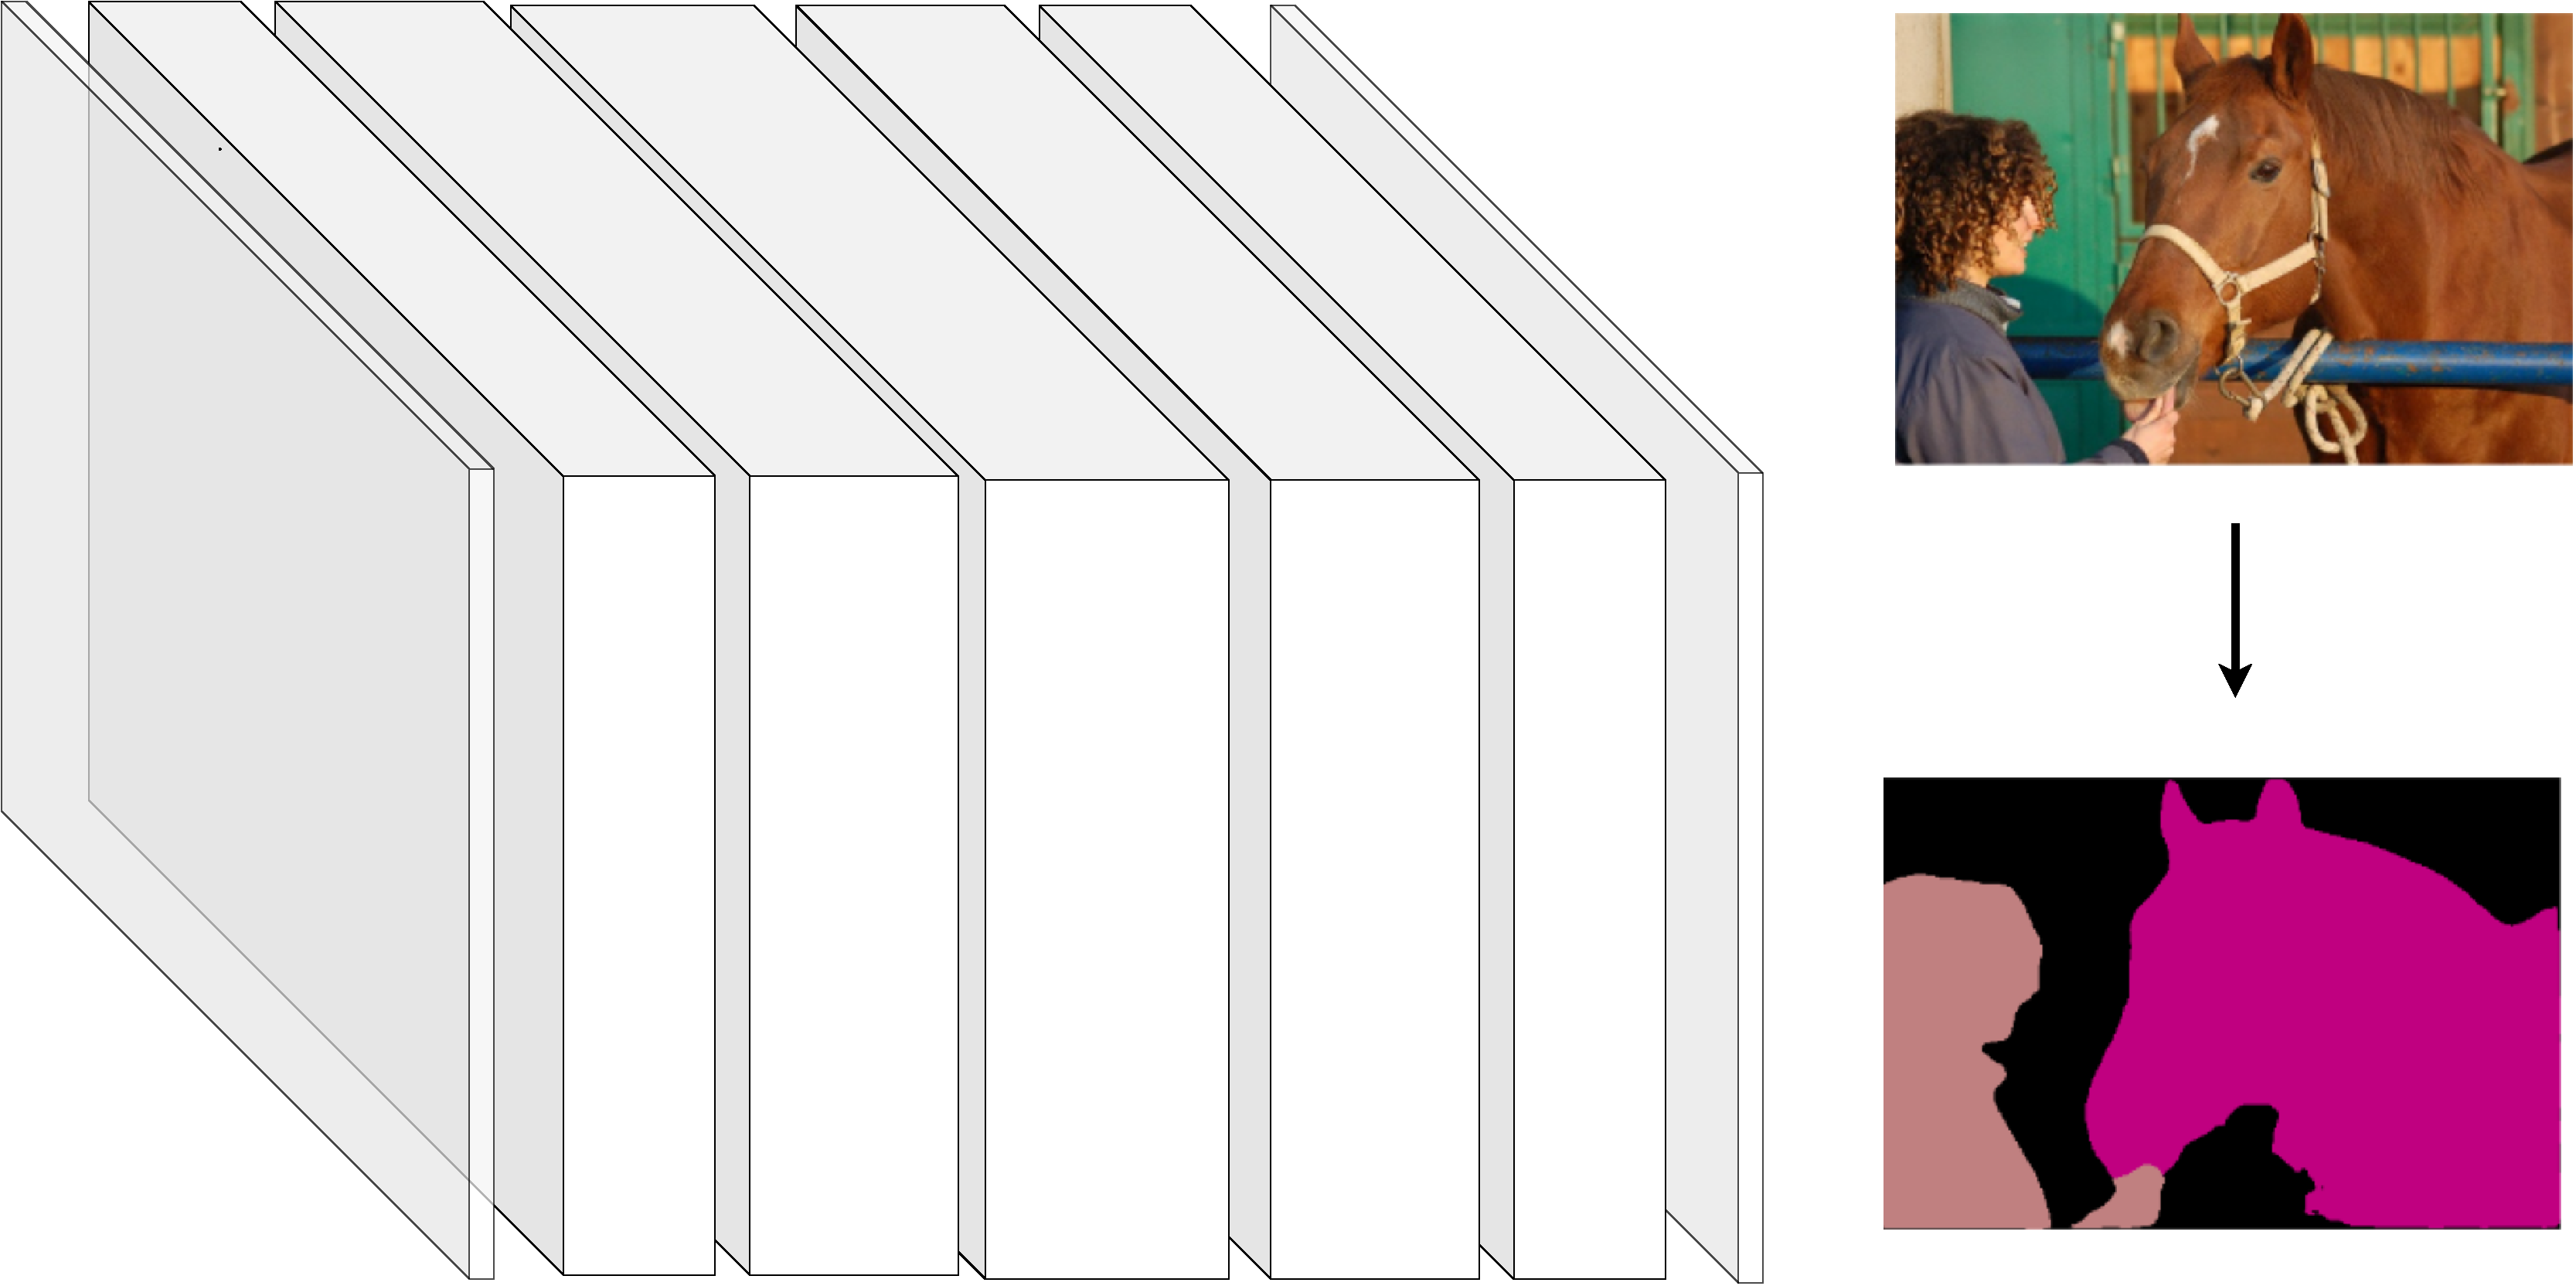
\includegraphics[width=0.9\textwidth]{segmentation_full}
  \end{figure}

  \note{
    \begin{itemize}
      \item Huge memory demands.
    \end{itemize}
  }
\end{frame}


\begin{frame}{Encoder-Decoder-Architecture}
  \begin{figure}
    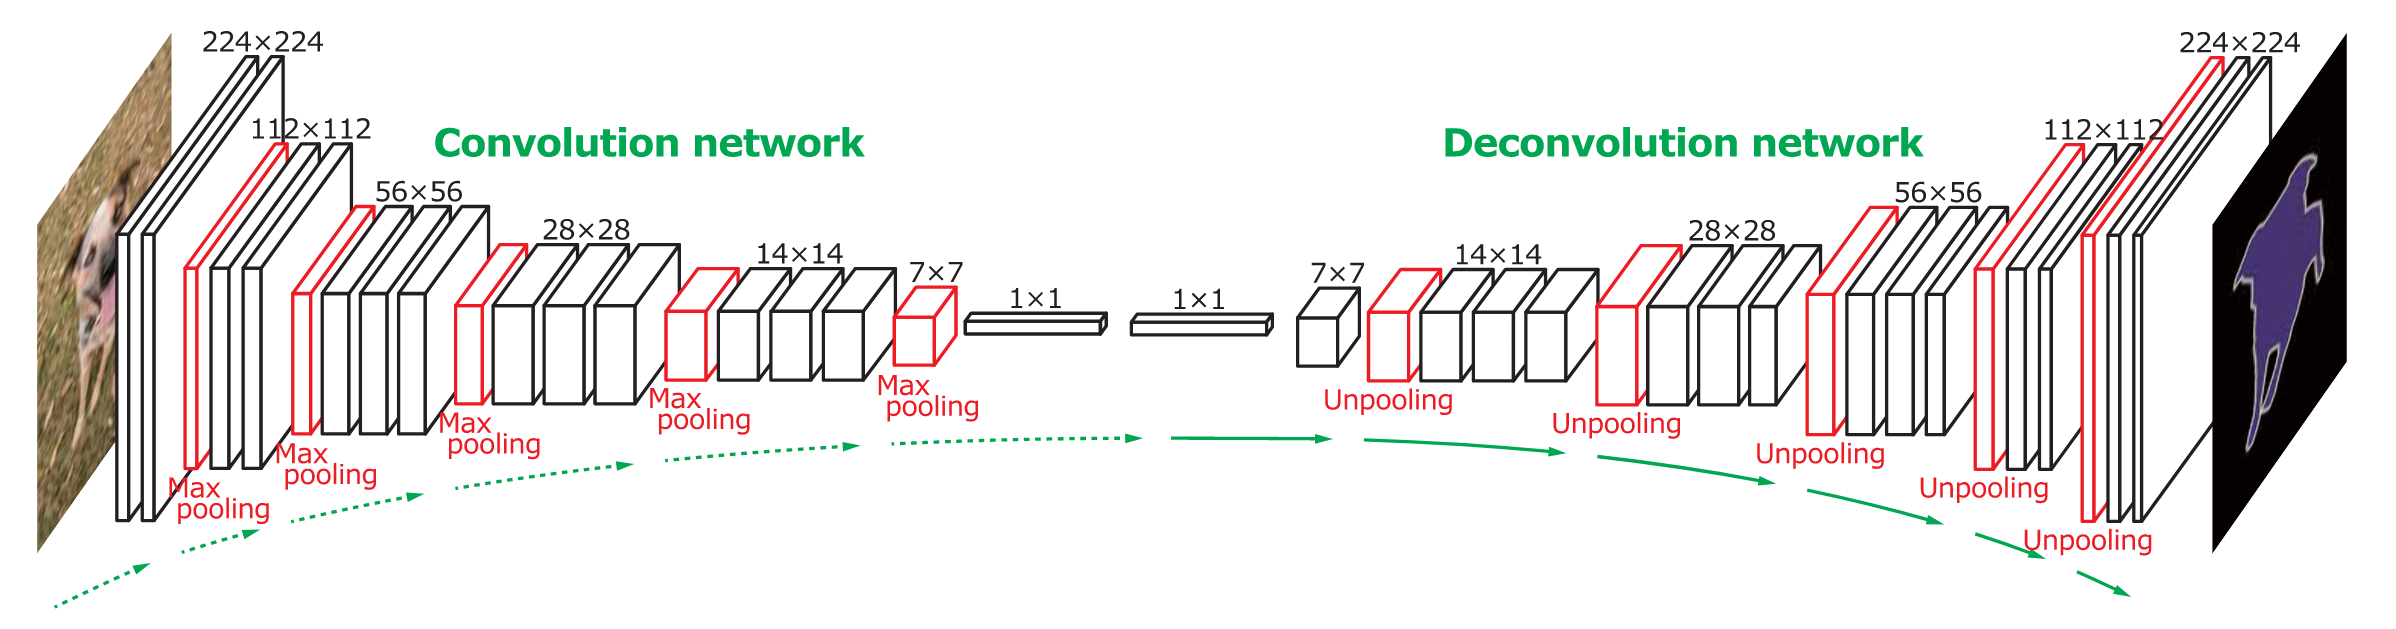
\includegraphics[width=0.9\textwidth]{encoder_decoder}
  \end{figure}
  \note{
    \begin{itemize}
      \item Image from Learning Deconvolution Network for Semantic Segmentation, Noh et al, ICCV 2015
    \end{itemize}
  }
\end{frame}


\begin{frame}{Unpooling}
  \begin{figure}
    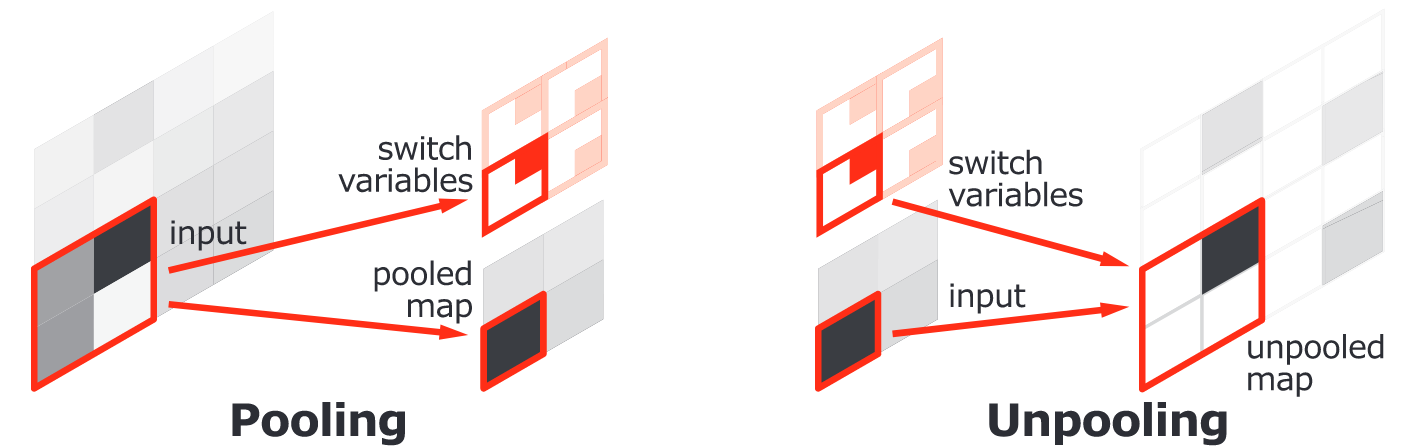
\includegraphics[width=0.9\textwidth]{pooling_unpooling}
  \end{figure}

  \note{
    \begin{itemize}
      \item Other unpooling methods: nearest neighbour or bed of nails.
      \item Image from Learning Deconvolution Network for Semantic Segmentation, Noh et al, ICCV 2015
    \end{itemize}
  }
\end{frame}


\begin{frame}{Deconvoluions}
  \begin{figure}
    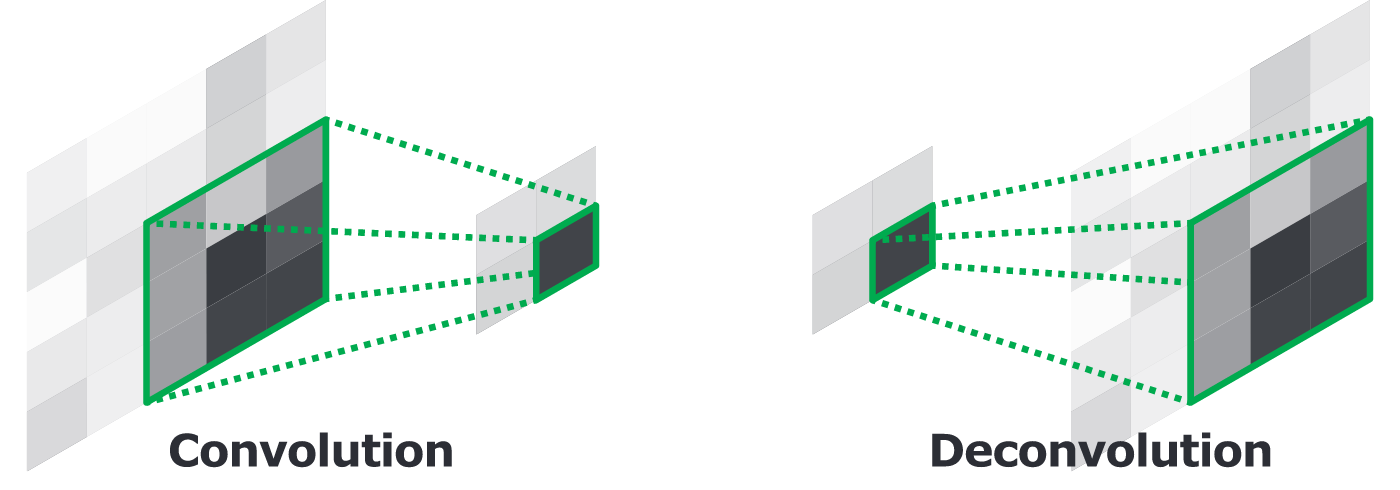
\includegraphics[width=0.9\textwidth]{conv_deconv}
  \end{figure}

  \note{
    \begin{itemize}
      \item Transpose convolution, deconvolution
      \item stride 2, pad 1, the other way
      \item Image from Learning Deconvolution Network for Semantic Segmentation, Noh et al, ICCV 2015
    \end{itemize}
  }
\end{frame}


\begin{frame}{Encoder-Decoder-Architecture}
  \begin{figure}
    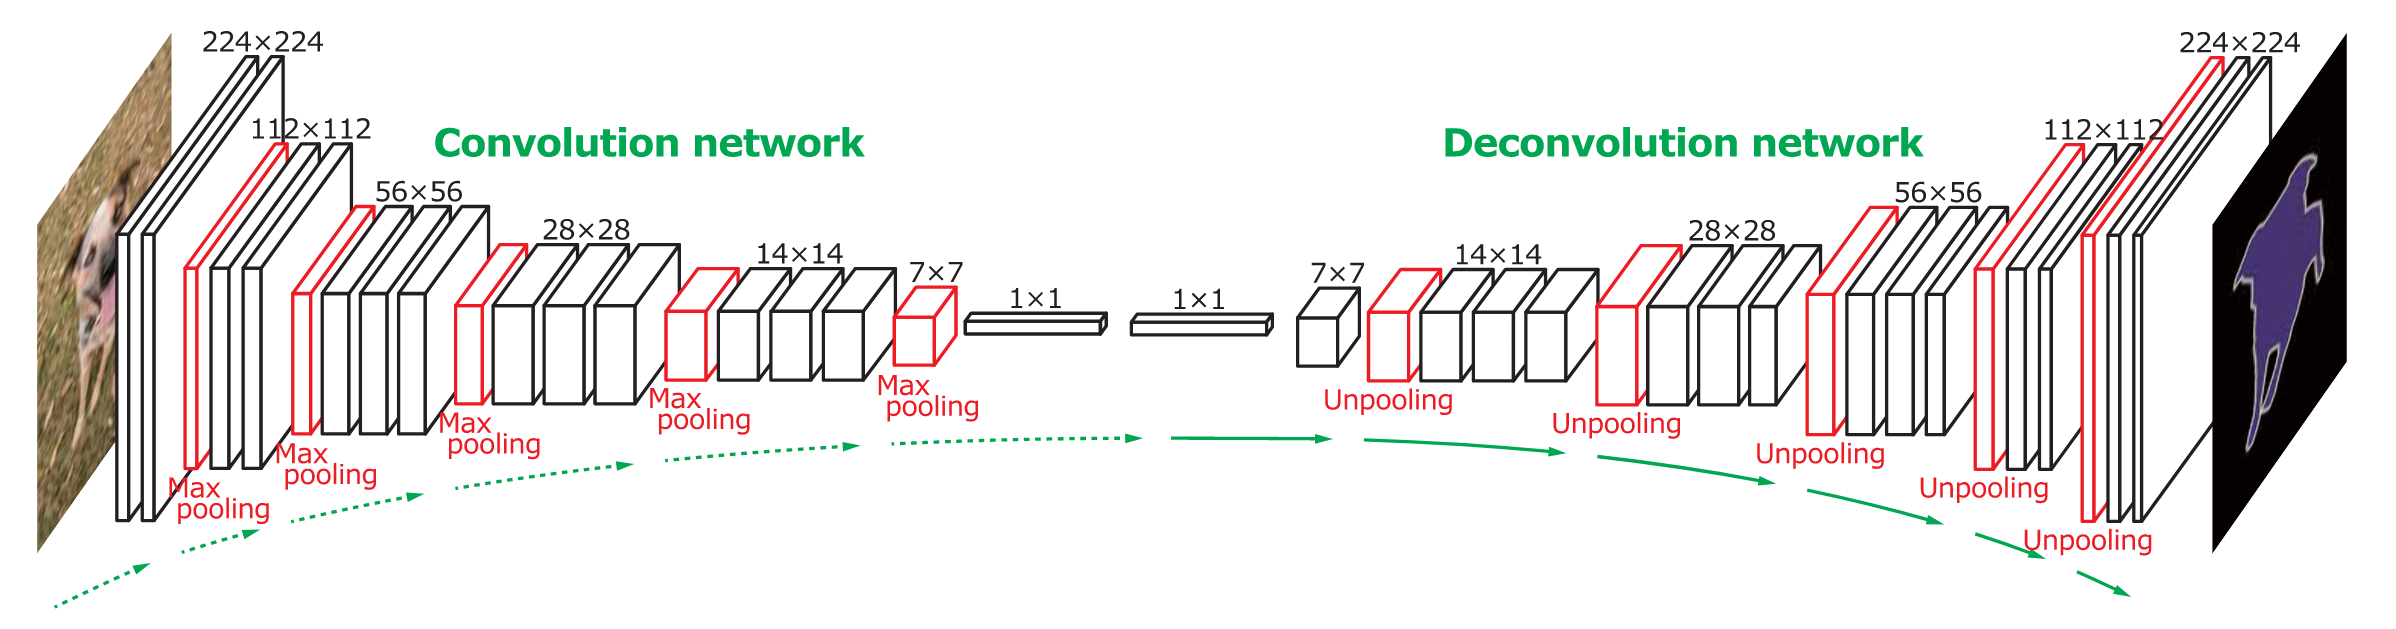
\includegraphics[width=0.9\textwidth]{encoder_decoder}
  \end{figure}
  \note{
    \begin{itemize}
      \item Problem: the coarse features (encoding in the middle) is supposed to be abstract and to not contain detailed geometrical information.
      \item Image from Learning Deconvolution Network for Semantic Segmentation, Noh et al, ICCV 2015
    \end{itemize}
  }
\end{frame}


\begin{frame}{UNet/Segnet}
  \begin{figure}
    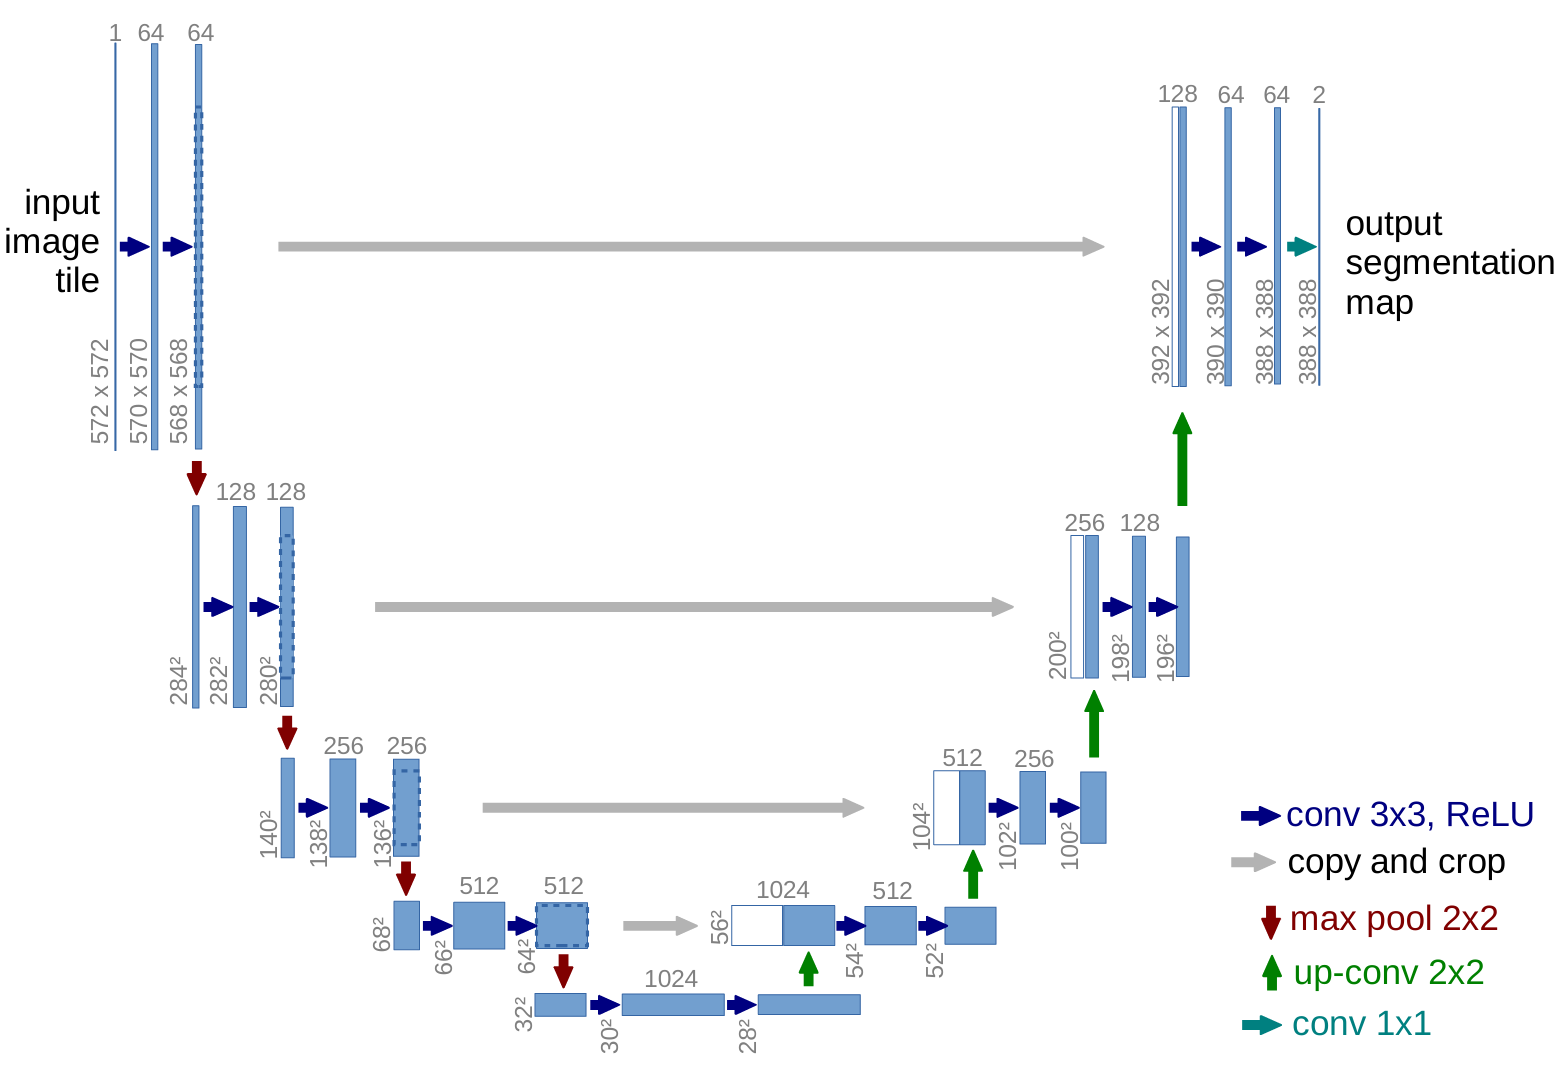
\includegraphics[width=0.55\textwidth]{unet}
  \end{figure}

  \note{
    \begin{itemize}
      \item Solution: skip connection.
      \item Image from U-Net: Convolutional Networks for Biomedical Image Segmentation, Ronnenberger et al, MICCAI 2015
      \item SegNet: A Deep Convolutional Encoder-Decoder Architecture for Image Segmentation,  Badrinarayanan et al, TPAMI 2017
    \end{itemize}
  }
\end{frame}


\begin{frame}{Pyramid Pooling}
  \begin{figure}
    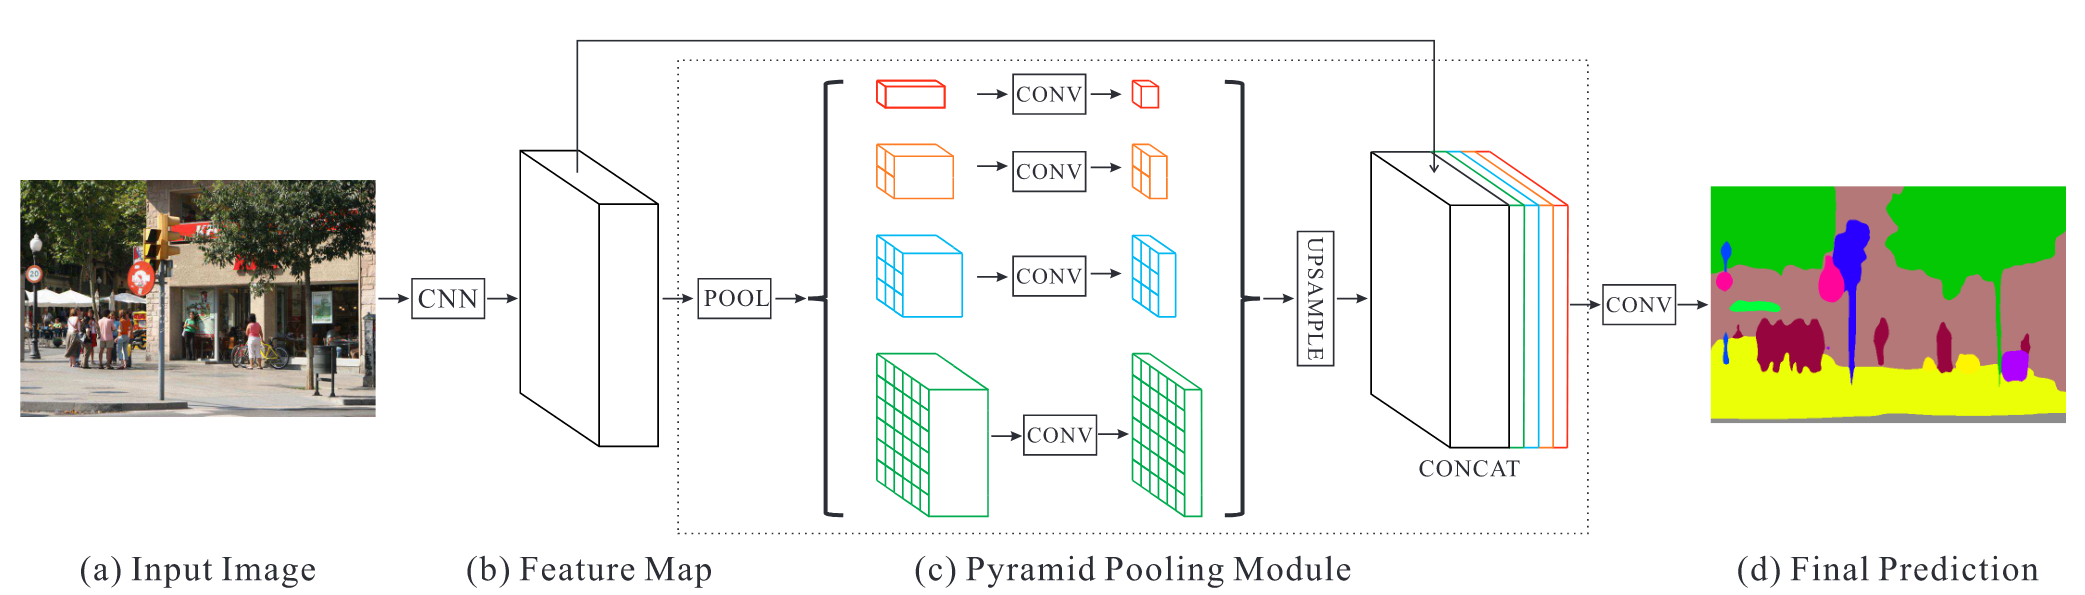
\includegraphics[width=0.9\textwidth]{pyramid_pooling}
  \end{figure}

  \note{
    \begin{itemize}
      \item Global context prior: to allow the network to process the image on different scales improves results.
      \item Improves the models ability to learn spatial semantics (spatial class co-occurence and spatial coherence).
      \item Improves recognition of very small object and stuff classes that exceed receptive fields.
      \item Image from Pyramid Scene Parsing Network, Zhao et al, CVPR 2017
    \end{itemize}
  }
\end{frame}


\begin{frame}{Pyramid Pooling: DeepLabv3+}
  \begin{figure}
    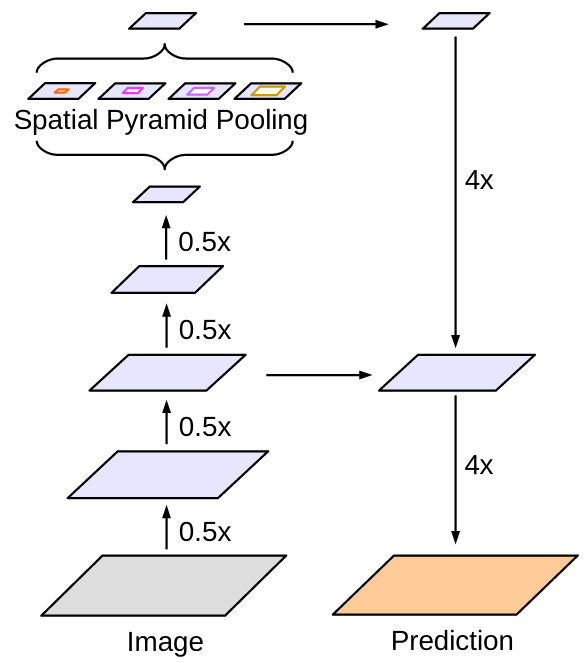
\includegraphics[width=0.45\textwidth]{deeplabv3p}
  \end{figure}

  \note{
    \begin{itemize}
      \item Case study of a SOTA semantic segmentation network: uses pretrained encoder network plus spatial pyramid pooling and skip connections.
      \item Image from Encoder-Decoder with Atrous Separable Convolution for Semantic Image Segmentation, Chen et al, ECCV 2018
    \end{itemize}
  }
\end{frame}

\begin{frame}{Object Detection}
  \begin{figure}
    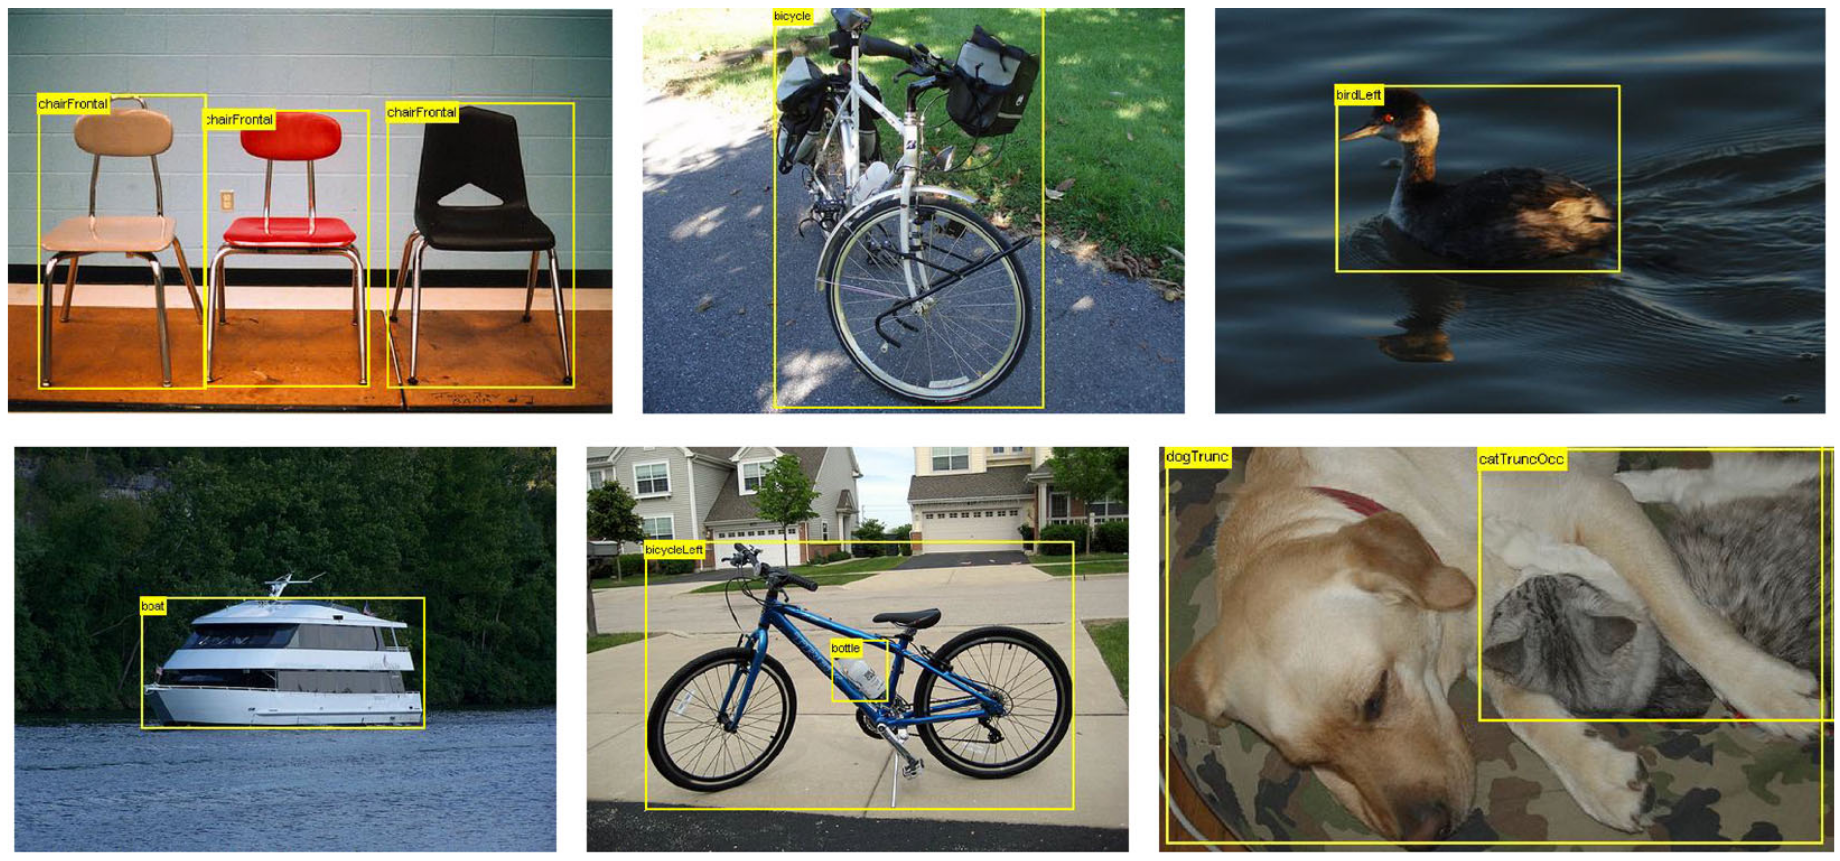
\includegraphics[width=0.9\textwidth]{detection_pascal_voc}
  \end{figure}

  \note{
    \begin{itemize}
      \item Image from The PASCAL Visual Object Classes Challenge: A Retrospective, Everingham et al, IJCV 2014
    \end{itemize}
  }
\end{frame}


\begin{frame}{Dataset: PASCAL Visual Object Classes}
  \begin{columns}
    \begin{column}{0.48\textwidth}
      \begin{figure}
        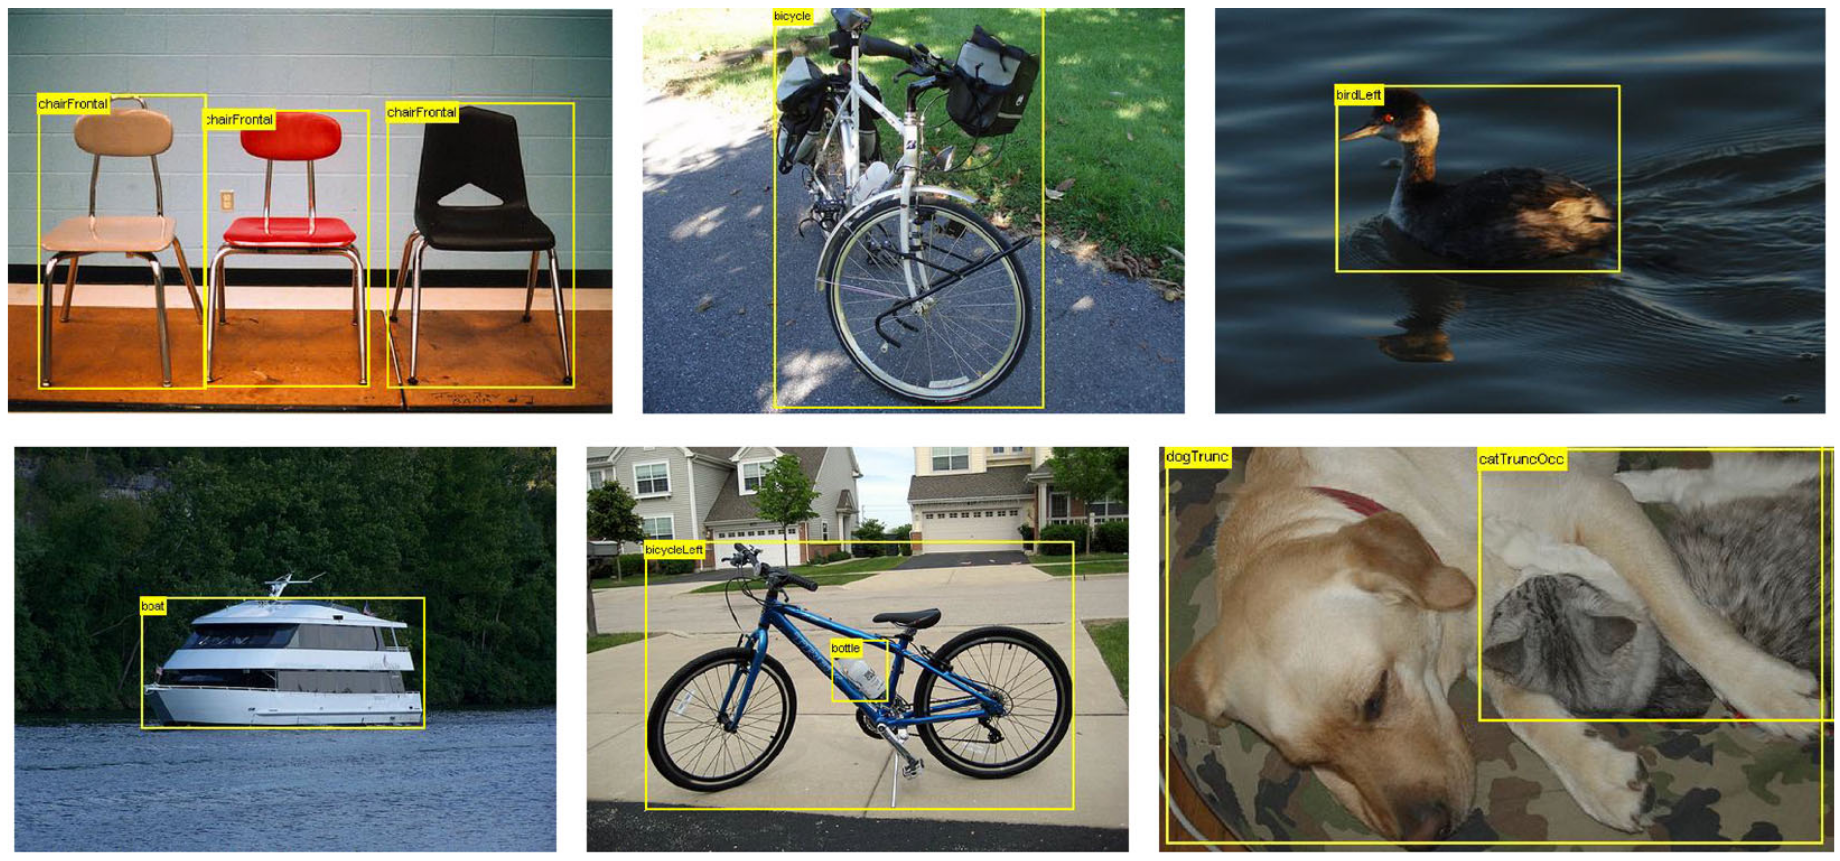
\includegraphics[width=0.9\textwidth]{detection_pascal_voc}
      \end{figure}
    \end{column}
    \begin{column}{0.48\textwidth}
    \begin{itemize}
      \item 20 classes
      \item 11k annotated images
      \item 27k annotated objects
    \end{itemize}

    \end{column}
  \end{columns}

  \note{
    \begin{itemize}
      \item Pascal VOC (DPM 33.6\%)
    \end{itemize}
  }
\end{frame}


\begin{frame}{Intersection over Union}
  Detection is correct if
  $$ intersection/union > threshold$$

  \begin{figure}
    
\includegraphics[width=0.9\textwidth]{iou}
  \end{figure}
  \note{
    \begin{itemize}
      \item Default threshold was 0.5 for a long time but is now often higher.
    \end{itemize}
  }
\end{frame}


\begin{frame}{Recall and Precision}
  \begin{align*}
    precision &= \nicefrac{\#(correct~detections)}{\#(all~detections)}\\
    recall &= \nicefrac{\#(correct~detections)}{\#(all~objects)} \\
  \end{align*}
      Average Precision: area under PR curve for specific class\\
      mean Average Precision: AP averaged over all classes
  \begin{figure}
    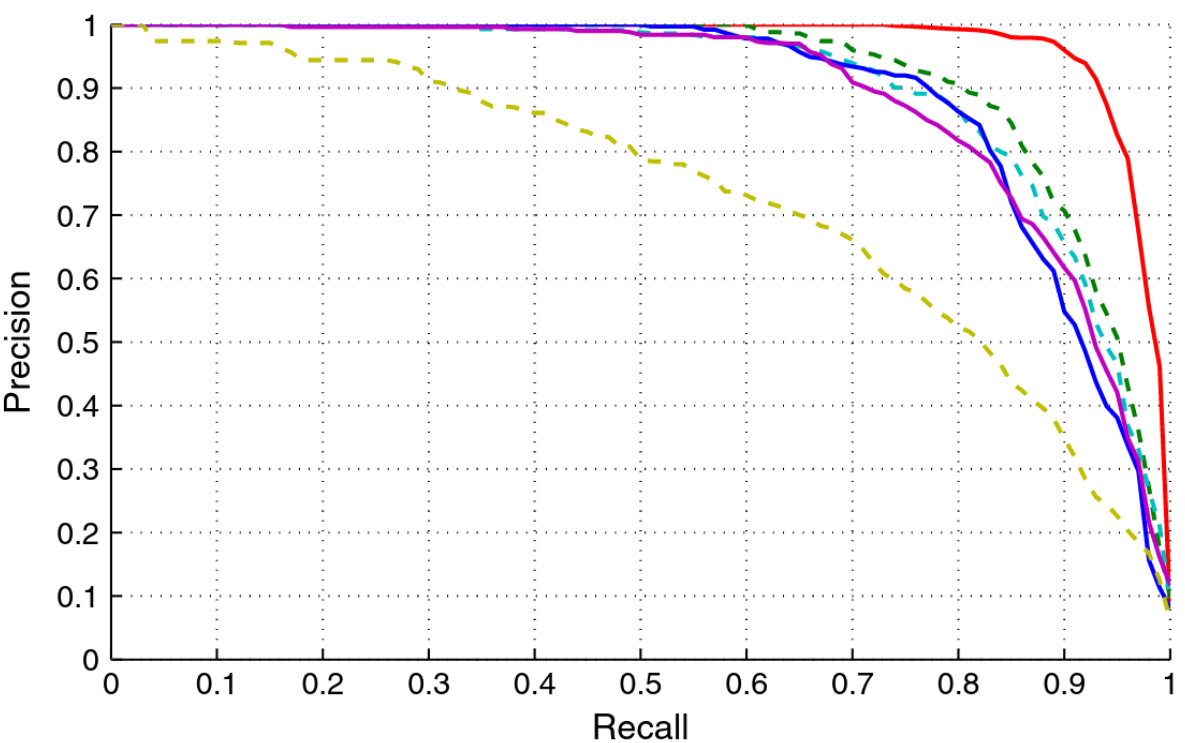
\includegraphics[width=0.5\textwidth]{precision_recall}
  \end{figure}

  \note{
    \begin{itemize}
      \item Image from The PASCAL Visual Object Classes Challenge: A Retrospective, Everingham et al, IJCV 2014
    \end{itemize}
  }
\end{frame}


\begin{frame}{Object Detection: output dimensionality?}
  \begin{figure}
    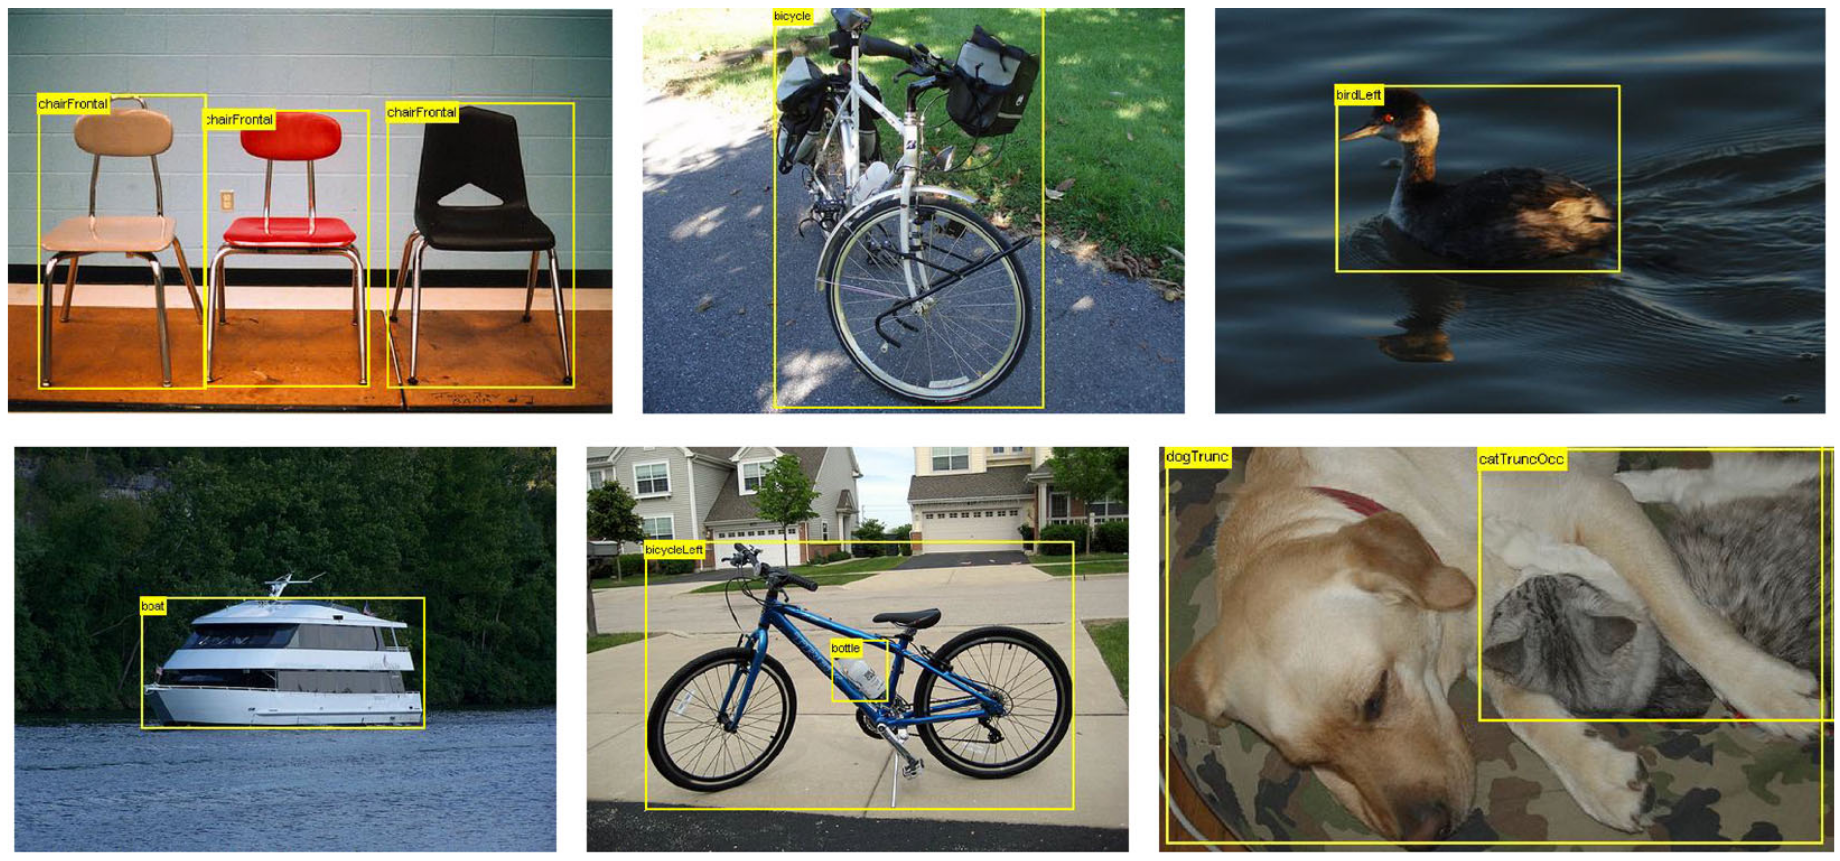
\includegraphics[width=0.9\textwidth]{detection_pascal_voc}
  \end{figure}

  \note{
    \begin{itemize}
      \item How would the head of this network look like?
      \item Image from The PASCAL Visual Object Classes Challenge: A Retrospective, Everingham et al, IJCV 2014
    \end{itemize}
  }
\end{frame}


\begin{frame}{R-CNN}
  \begin{figure}
    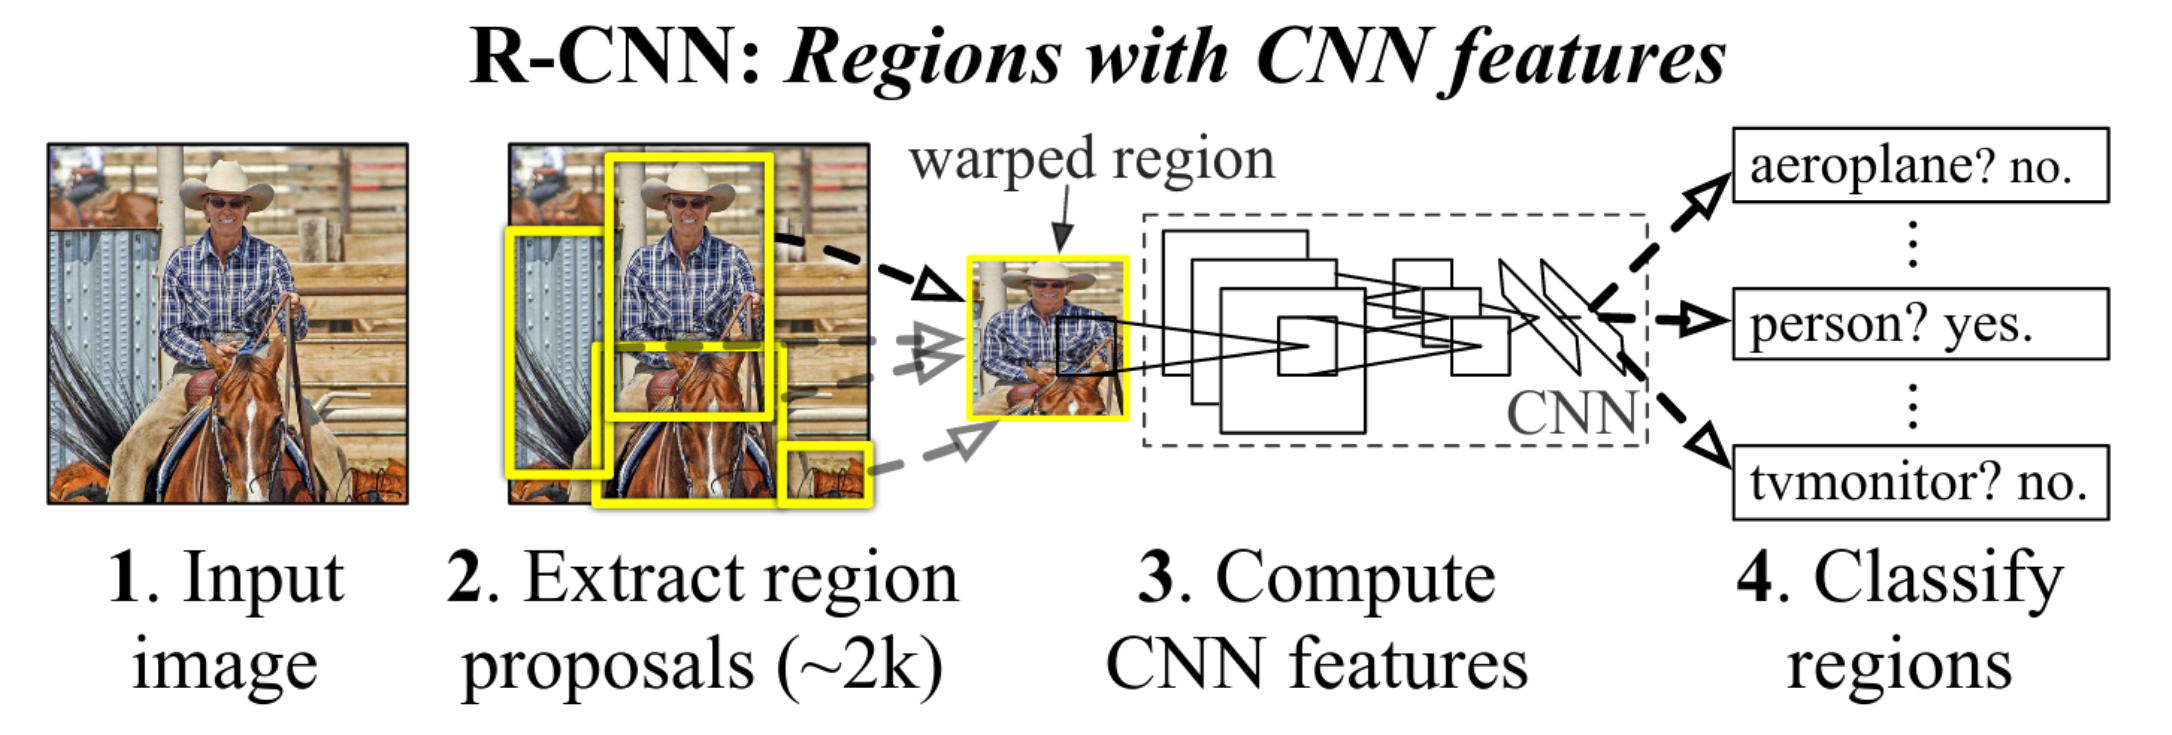
\includegraphics[width=0.9\textwidth]{rcnn}
  \end{figure}

  \note{
    \begin{itemize}
      \item Same author as DPM.
      \item Sliding window as in DPM. But NN much slower as SVM, therefore they used region proposals (2k).
      \item Image from Rich feature hierarchies for accurate object detection and semantic segmentation, Girshick et al, CVPR 2014
    \end{itemize}
  }
\end{frame}


\begin{frame}{Region Proposals}
  \begin{figure}
    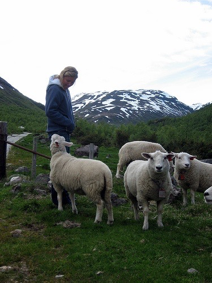
\includegraphics[width=0.15\textwidth]{selective_search_01}
    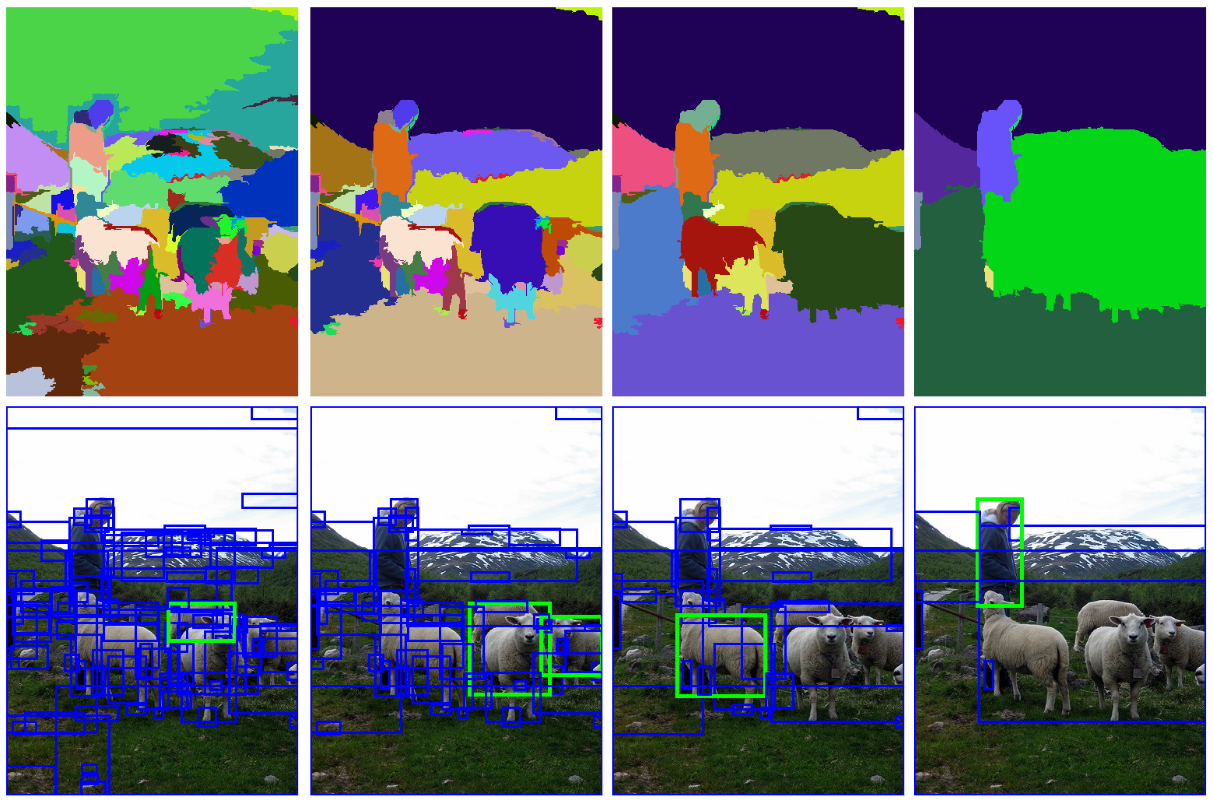
\includegraphics[width=0.65\textwidth]{selective_search_00}
  \end{figure}

  \note{
    \begin{itemize}
      \item Image from Selective Search for Object Recognition, Uijlings et al, IJCV 2013
    \end{itemize}
  }
\end{frame}


\begin{frame}{R-CNN}
  \begin{figure}
    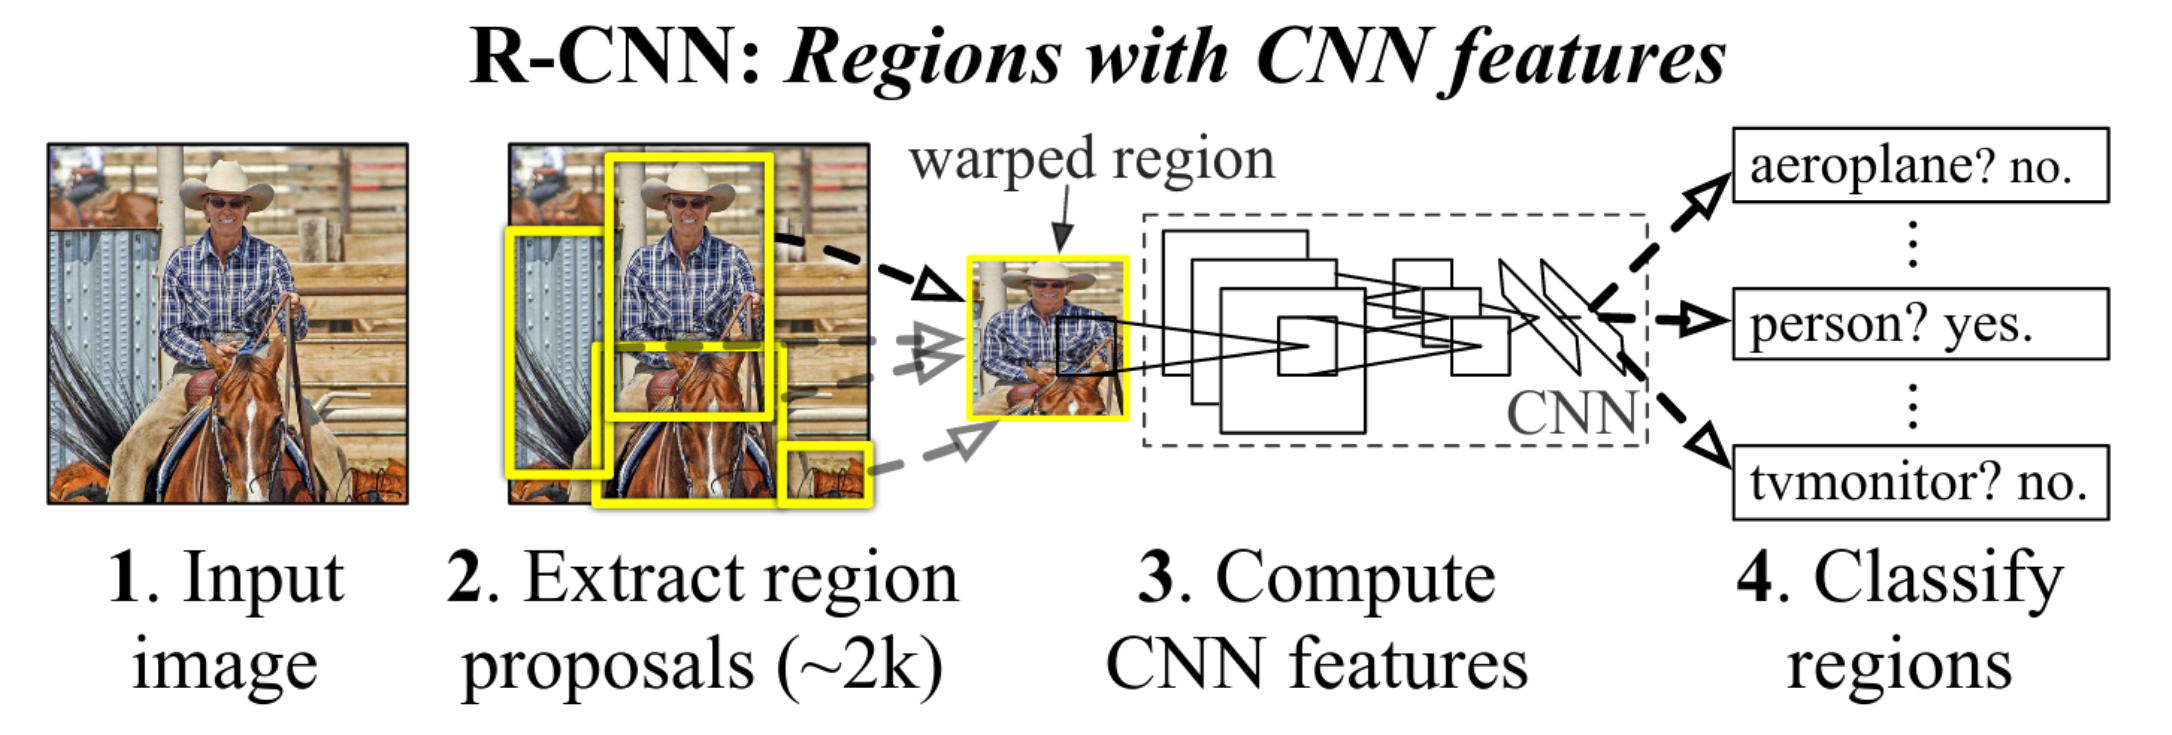
\includegraphics[width=0.9\textwidth]{rcnn}
  \end{figure}

  \note{
    \begin{itemize}
      \item Network also needs to predict bounding box parameters (size and offset from patch center).
      \item Non maximum suppression in prediction space.
      \item Often some high level reasoning (coherence in object relations).
      \item mAP for Pascal VOC improved to 53\% with AlexNet as ConvNet and 62\% with VGG (from 33\% DPM)
      \item Image from Rich feature hierarchies for accurate object detection and semantic segmentation, Girshick et al, CVPR 2014
    \end{itemize}
  }
\end{frame}


\begin{frame}{Fast-RCNN}
  \begin{figure}
    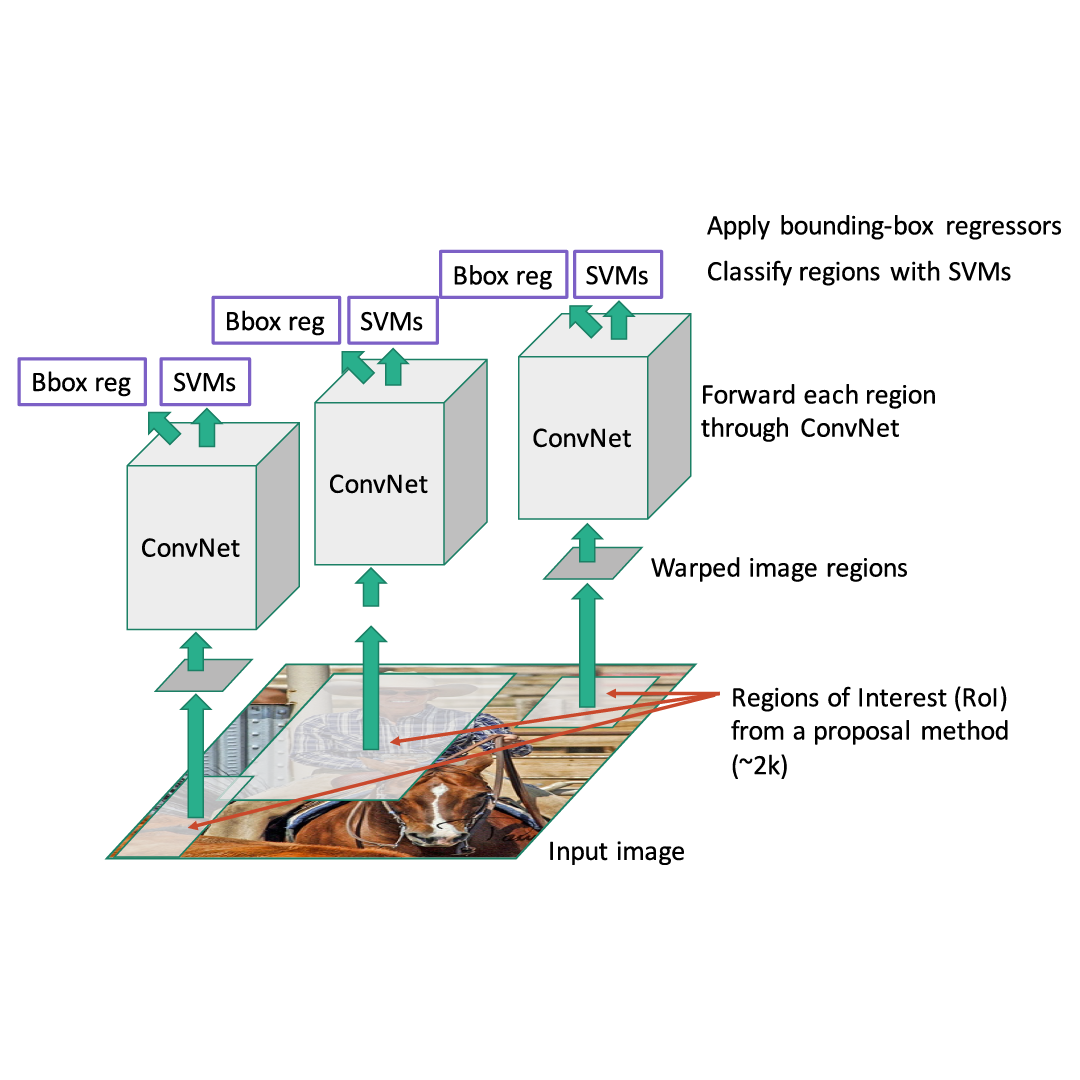
\includegraphics[width=0.45\textwidth]{slow_rcnn}
    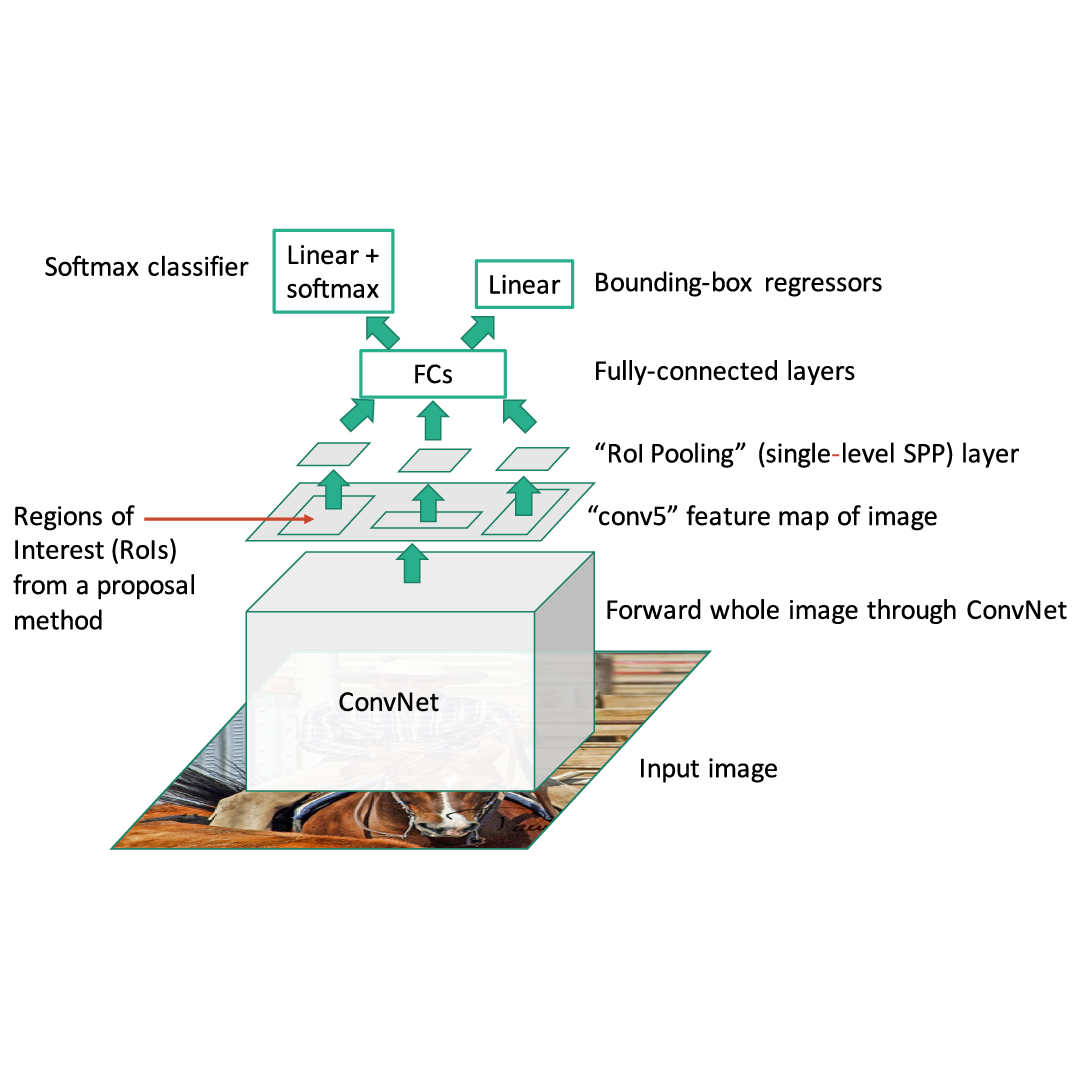
\includegraphics[width=0.45\textwidth]{fast_rcnn}
  \end{figure}

  \note{
    \begin{itemize}
      \item Moves the cropping of proposed regions to the feature map, saving the many forward passes through the convolutional block.
      \item Image from Talk at ICCV 2015 by Ross Girshick \url{https://dl.dropboxusercontent.com/s/vlyrkgd8nz8gy5l/fast-rcnn.pdf?dl=0}
    \end{itemize}
  }
\end{frame}


% \begin{frame}{ROI Pooling}
%   \note{
%     \begin{itemize}
%       \item
%     \end{itemize}
%   }
% \end{frame}


% \begin{frame}{ROI Align}
%   \note{
%     \begin{itemize}
%       \item
%     \end{itemize}
%   }
% \end{frame}



\begin{frame}{Faster-RCNN}
  \begin{figure}
    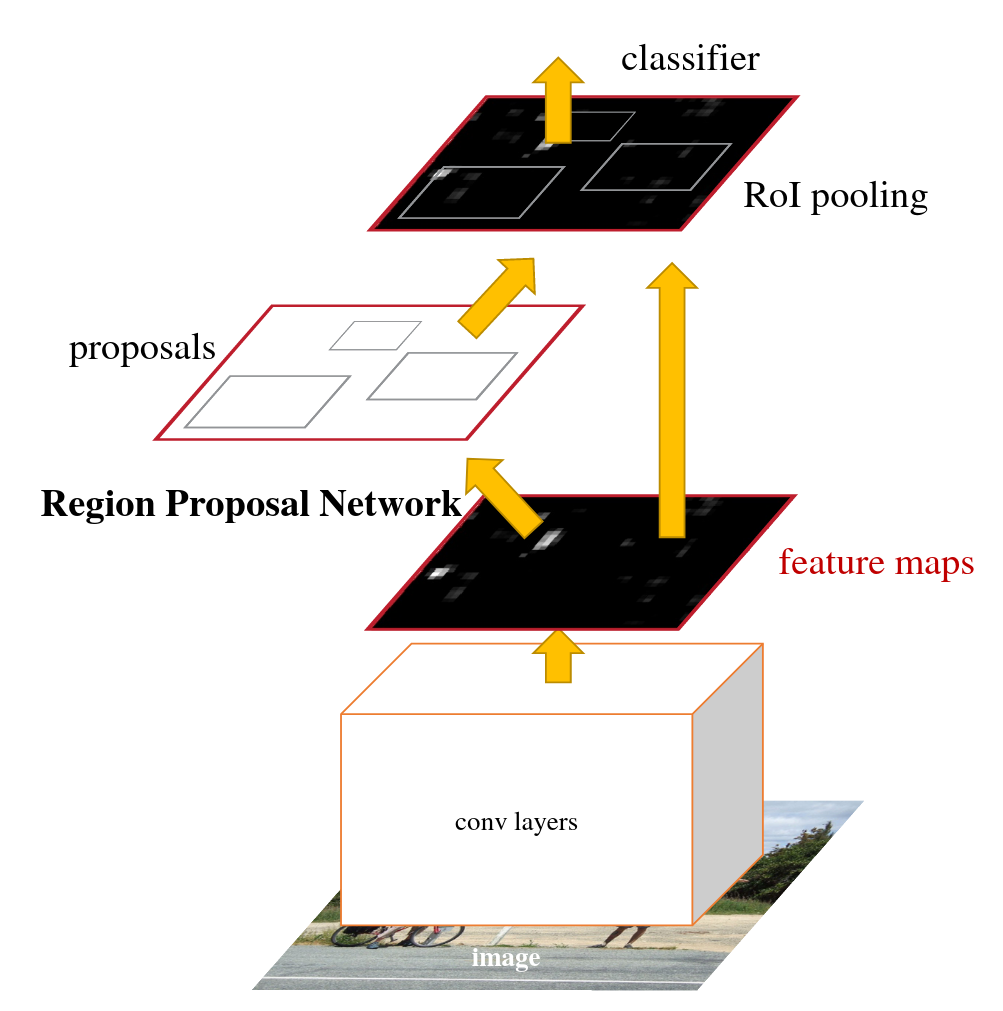
\includegraphics[width=0.5\textwidth]{faster_rcnn}
  \end{figure}

  \note{
    \begin{itemize}
      \item Region proposal is now the expensive step in Fast-RNN.
      \item Faster-RCNN does bounding box regression with a neural network based on the same image features the classifier uses, removing the region proposal step completely.
      \item Solution: Do region proposal in feature map.
    \end{itemize}
  }
\end{frame}


\begin{frame}{YOLO: You Only Look Once}
  \begin{figure}
    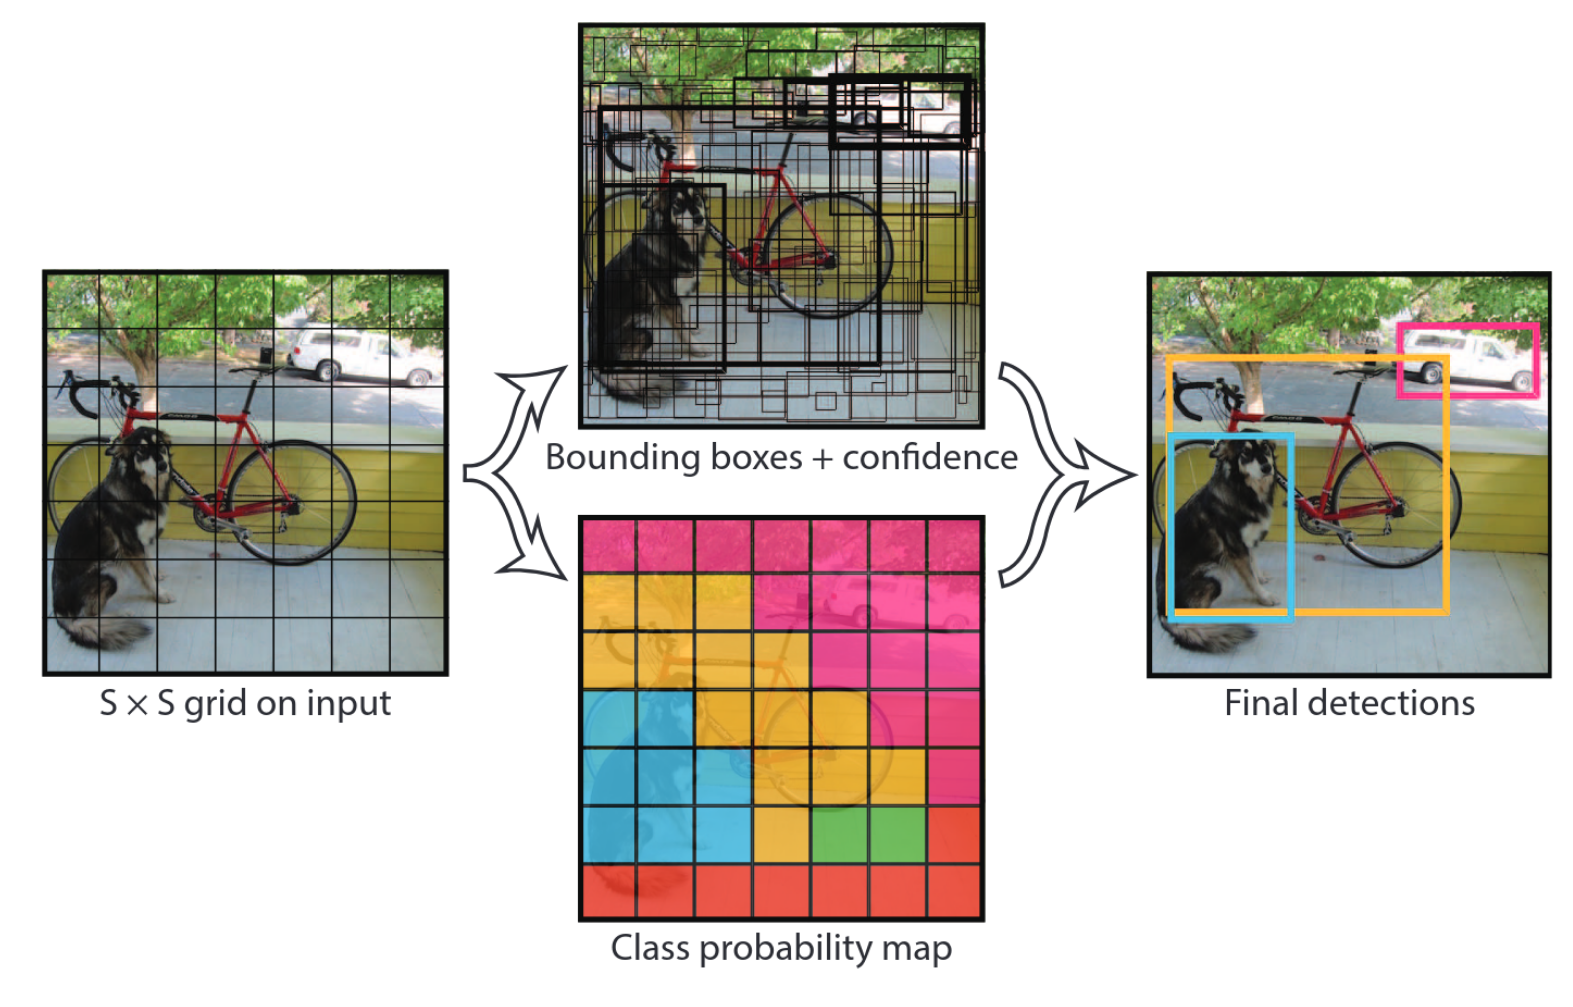
\includegraphics[width=0.8\textwidth]{yolo_00}
  \end{figure}

  \note{
    \begin{itemize}
      \item Image from You Only Look Once:Unified, Real-Time Object Detection, Redmon et al, CVPR 2016
    \end{itemize}
  }
\end{frame}


\begin{frame}{YOLO: You Only Look Once}
  \begin{figure}
    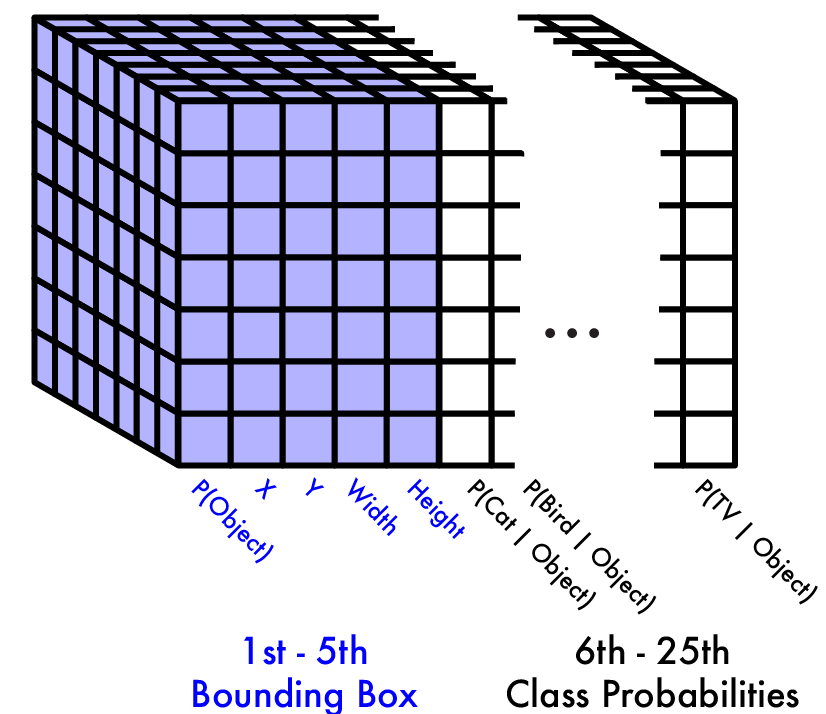
\includegraphics[width=0.55\textwidth]{yolo_01}
  \end{figure}

  \note{
    \begin{itemize}
      \item Newer versions of YOLO have multiple detections per cell for different object sizes.
      \item Image from Ancient Secrets of Computer Vision Lecture 18, Joseph Redmon
    \end{itemize}
  }
\end{frame}



\begin{frame}{YOLO: loss}
  \begin{align*}
    \mathcal{L} &= \alpha_{1}\mathcal{L}_{localization} + \alpha_{2}\mathcal{L}_{object~confidence} + \alpha_{3}\mathcal{L}_{classification} \\
    \mathcal{L}_{localization}&: root~mean~squared~error \\
    \mathcal{L}_{object~confidence}&: binary~cross~entropy \\
    \mathcal{L}_{classification}&: multi-class~cross~entropy
  \end{align*}
  \note{
    \begin{itemize}
      \item weighted loss, binary and multi-class cross entropy, MSE
      \item What would happen without conditional probability?
    \end{itemize}
  }
\end{frame}


% \begin{frame}{RetinaNet}
%   \note{
%     \begin{itemize}
%       \item
%       \item
%     \end{itemize}
%   }
% \end{frame}


\begin{frame}{Why not both? Instance Segmentation}
  \begin{figure}
    
\includegraphics[width=0.5\textwidth]{deeplabv3p_result_person}
    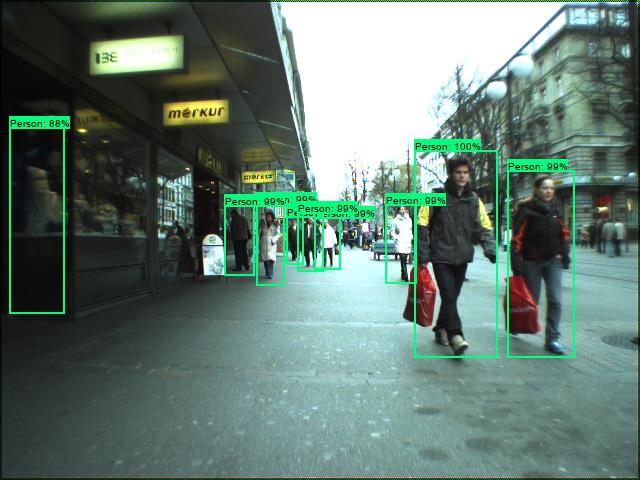
\includegraphics[width=0.4\textwidth]{detection_person}
  \end{figure}

  \note{
    \begin{itemize}
      \item Pixel level classification with instance boundaries.
    \end{itemize}
  }
\end{frame}


\begin{frame}{Mask R-CNN}
  \begin{figure}
    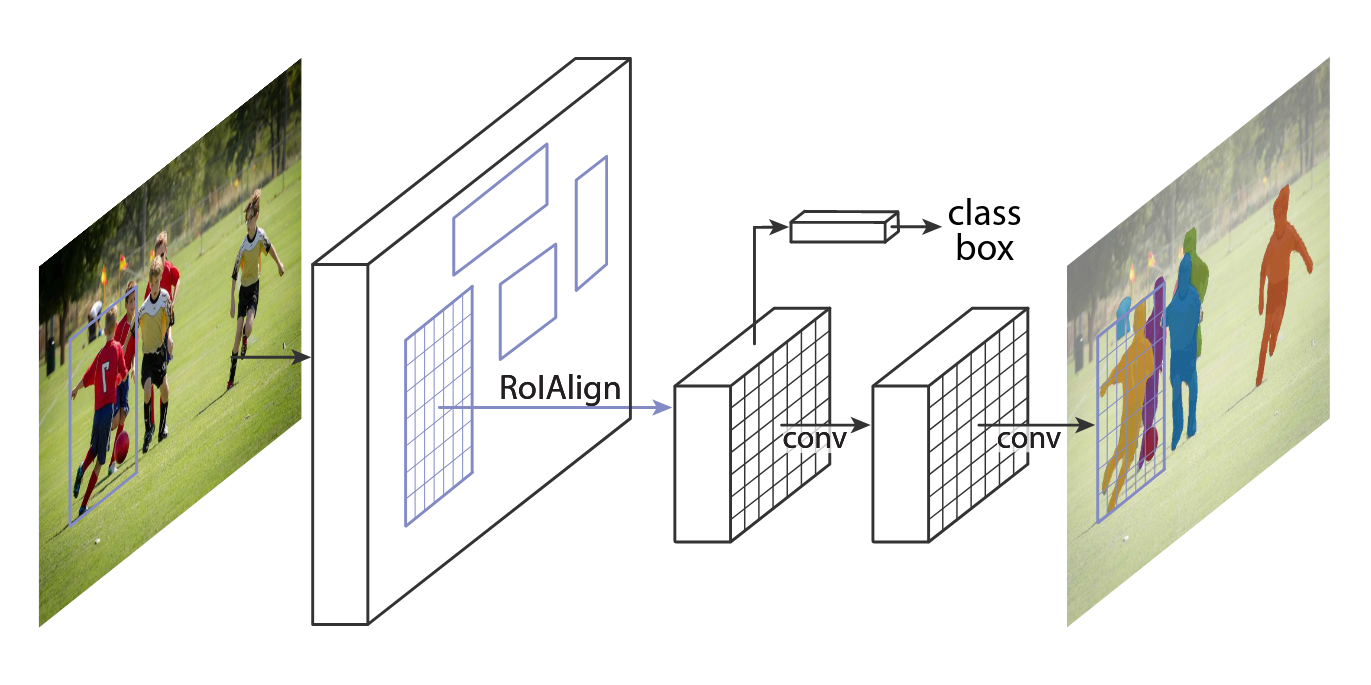
\includegraphics[width=0.9\textwidth]{mask_rcnn}
  \end{figure}

  \note{
    \begin{itemize}
      \item Faster R-CNN with segmentation network.
      \item Image from Mask R-CNN, He et al, ICCV 2017
    \end{itemize}
  }
\end{frame}


\begin{frame}{Mask R-CNN}
  \begin{figure}
    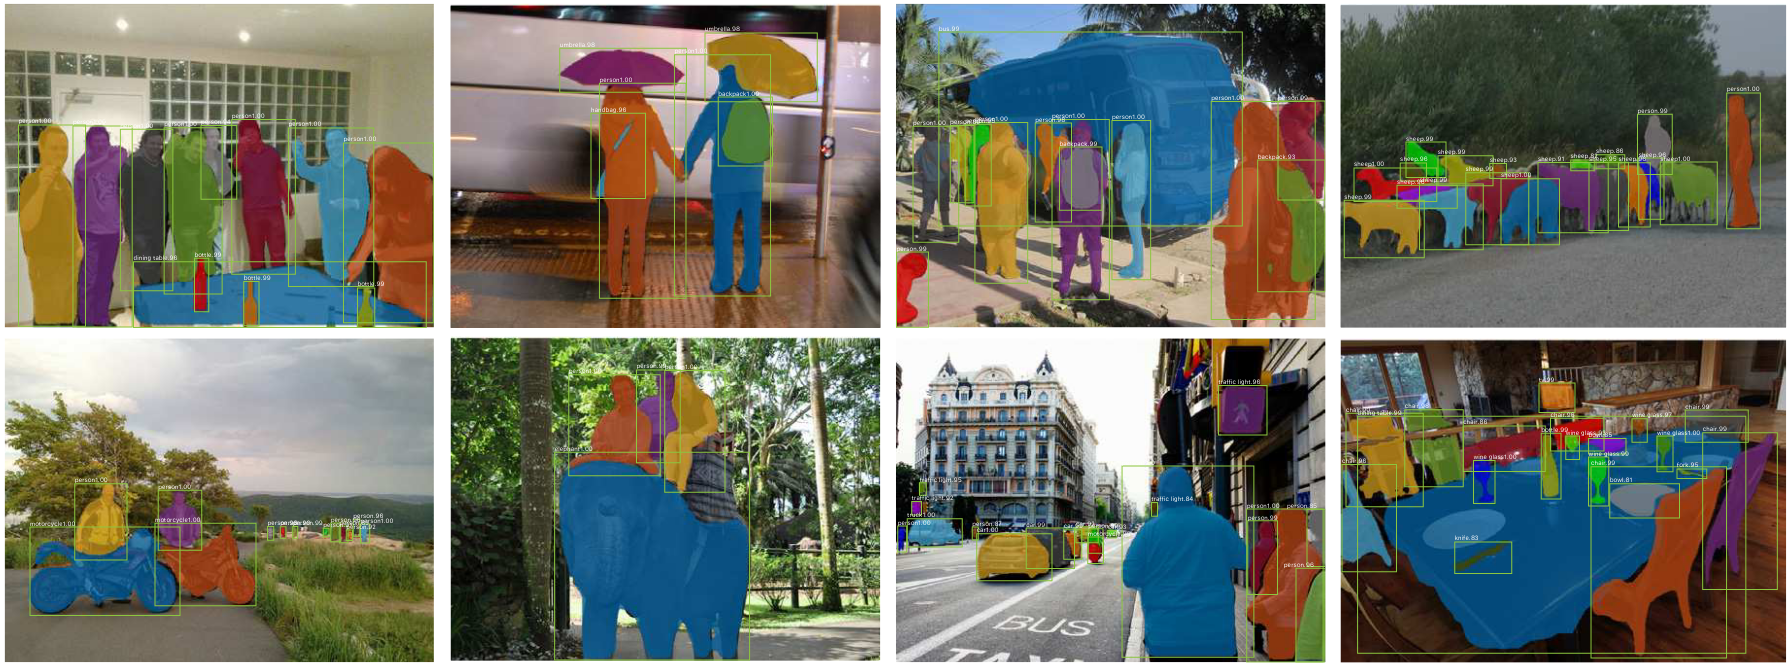
\includegraphics[width=0.9\textwidth]{mask_rcnn_results}
  \end{figure}

  \note{
    \begin{itemize}
      \item Results for Mask R-CNN.
      \item Image from Mask R-CNN, He et al, ICCV 2017
    \end{itemize}
  }
\end{frame}


\begin{frame}{Mask R-CNN}
  \begin{figure}
    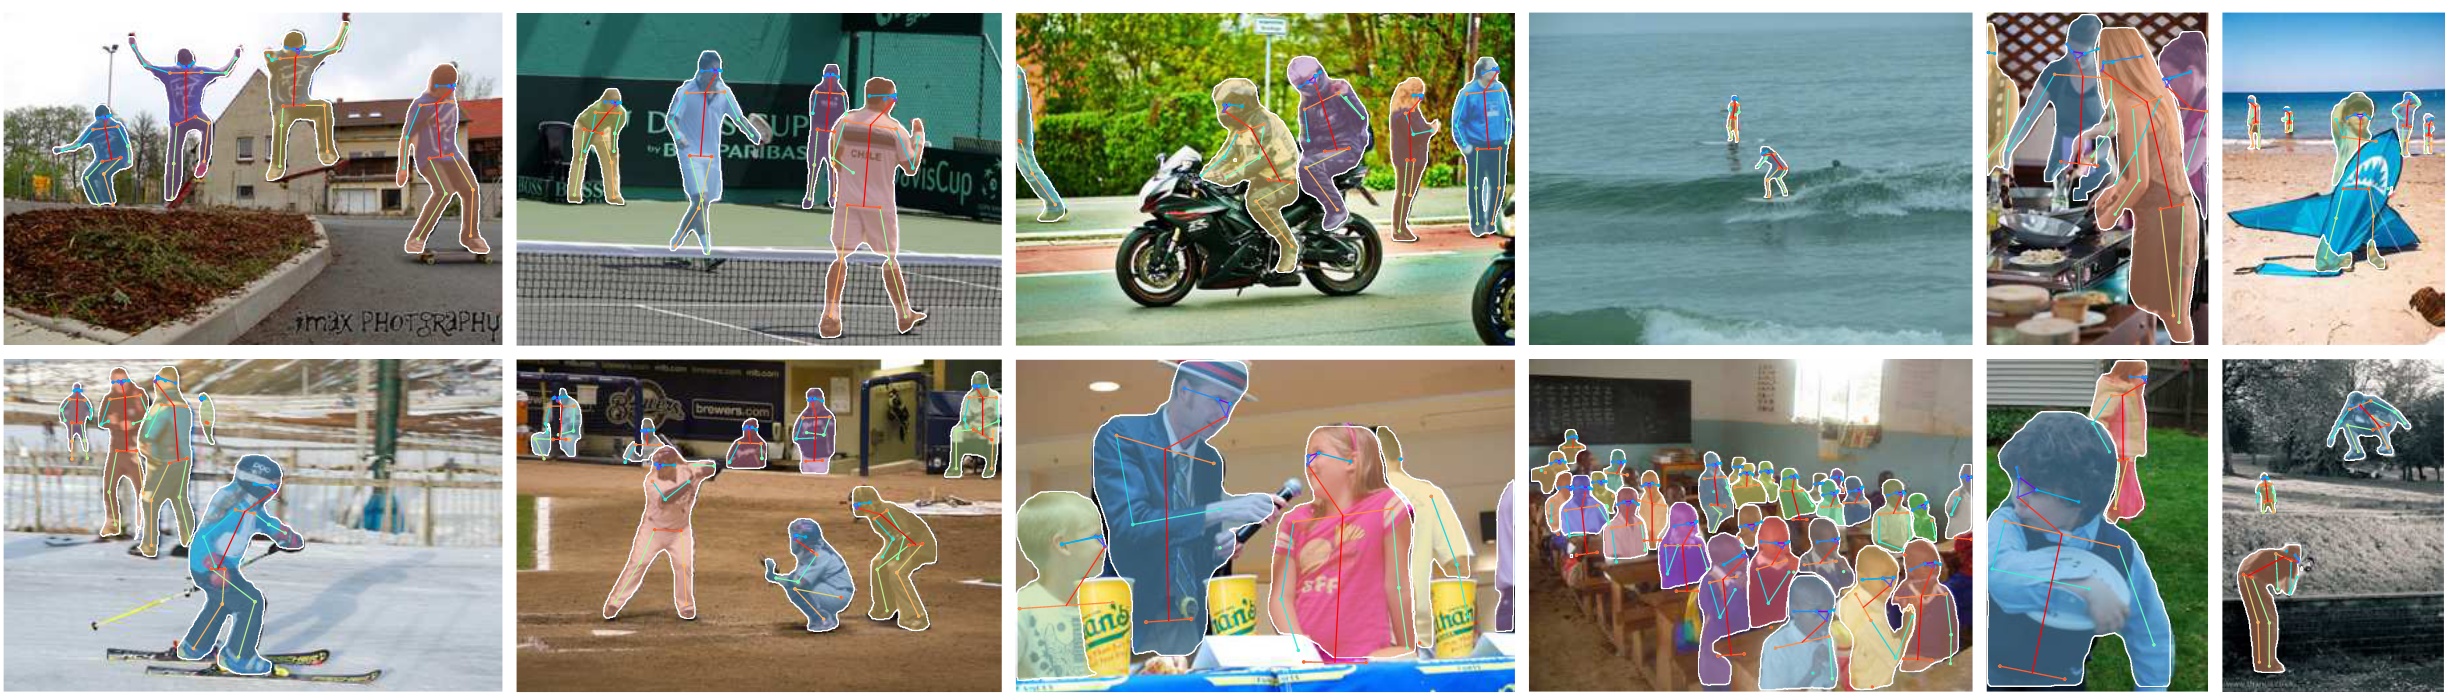
\includegraphics[width=0.9\textwidth]{mask_rcnn_keypoints}
  \end{figure}

  \note{
    \begin{itemize}
      \item Mask R-CNN can also learn skeletons.
      \item Image from Mask R-CNN, He et al, ICCV 2017
    \end{itemize}
  }
\end{frame}

\begin{frame}{Generalization}
  \begin{figure}
    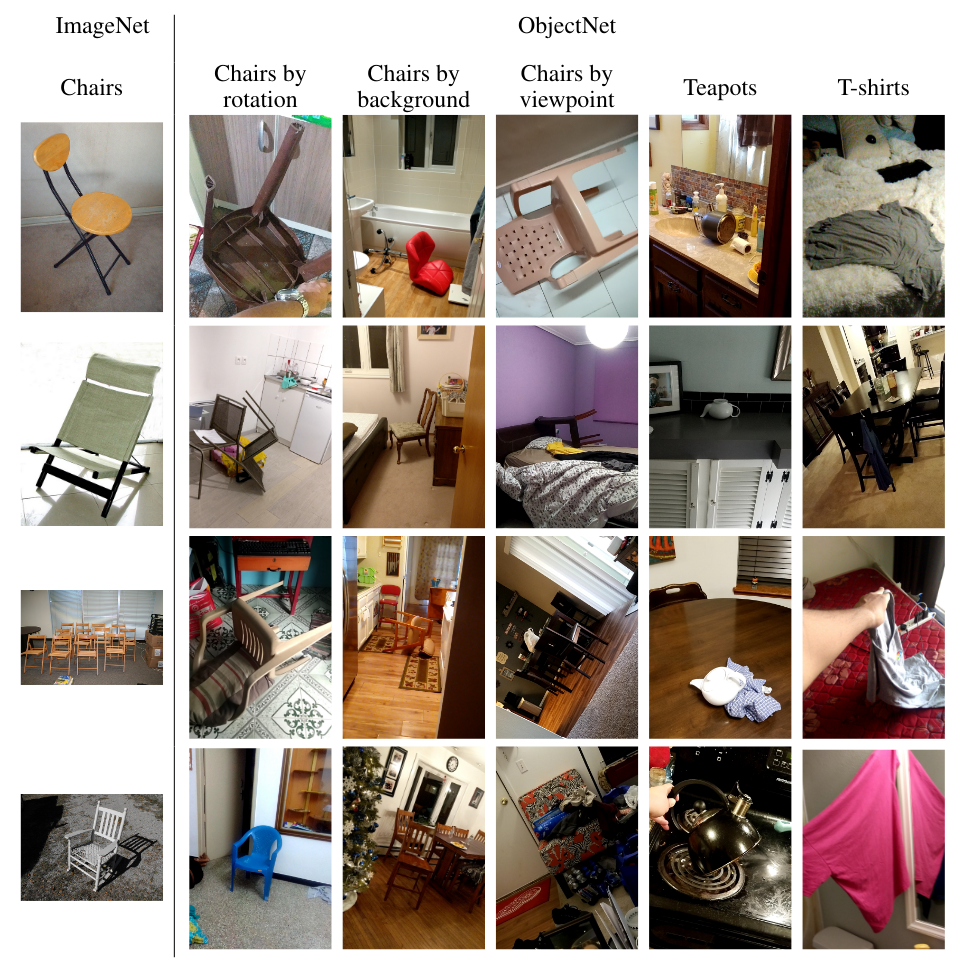
\includegraphics[width=0.4\textwidth]{objectnet_examples}
    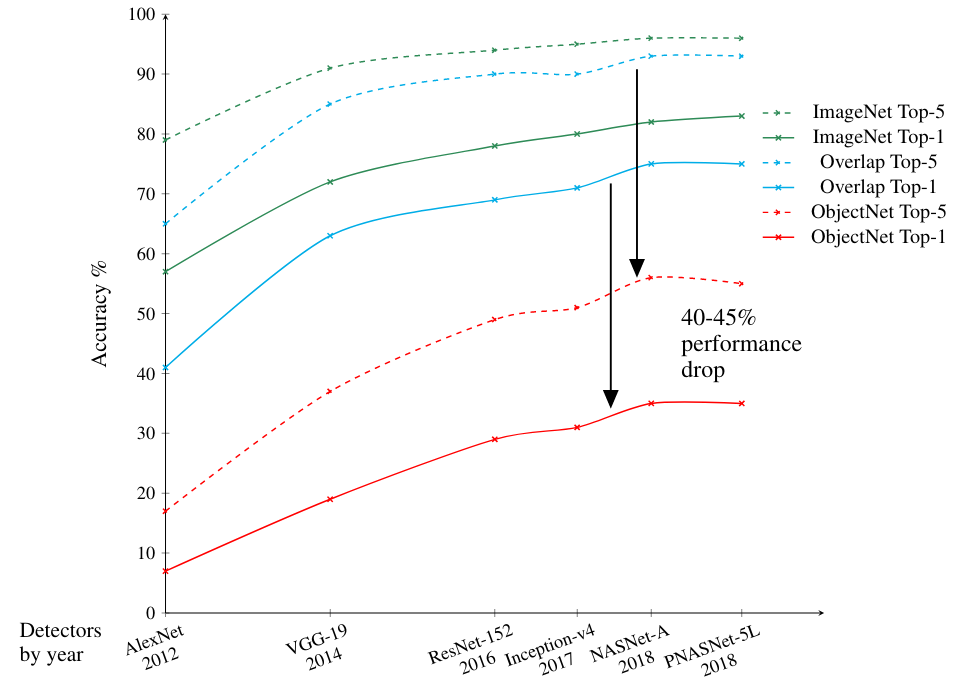
\includegraphics[width=0.55\textwidth]{objectnet_graph}
  \end{figure}

  \note{
    \begin{itemize}
      \item Neural Networks trained and evaluated on ImageNet do not generalize to o.o.d. data.
      \item Image from ObjectNet: A large-scale bias-controlled dataset forpushing the limits of object recognition models, Barbu et al, NeurIPS 2019
    \end{itemize}
  }
\end{frame}


\begin{frame}{Neural Networks are lazy}
  \begin{figure}
    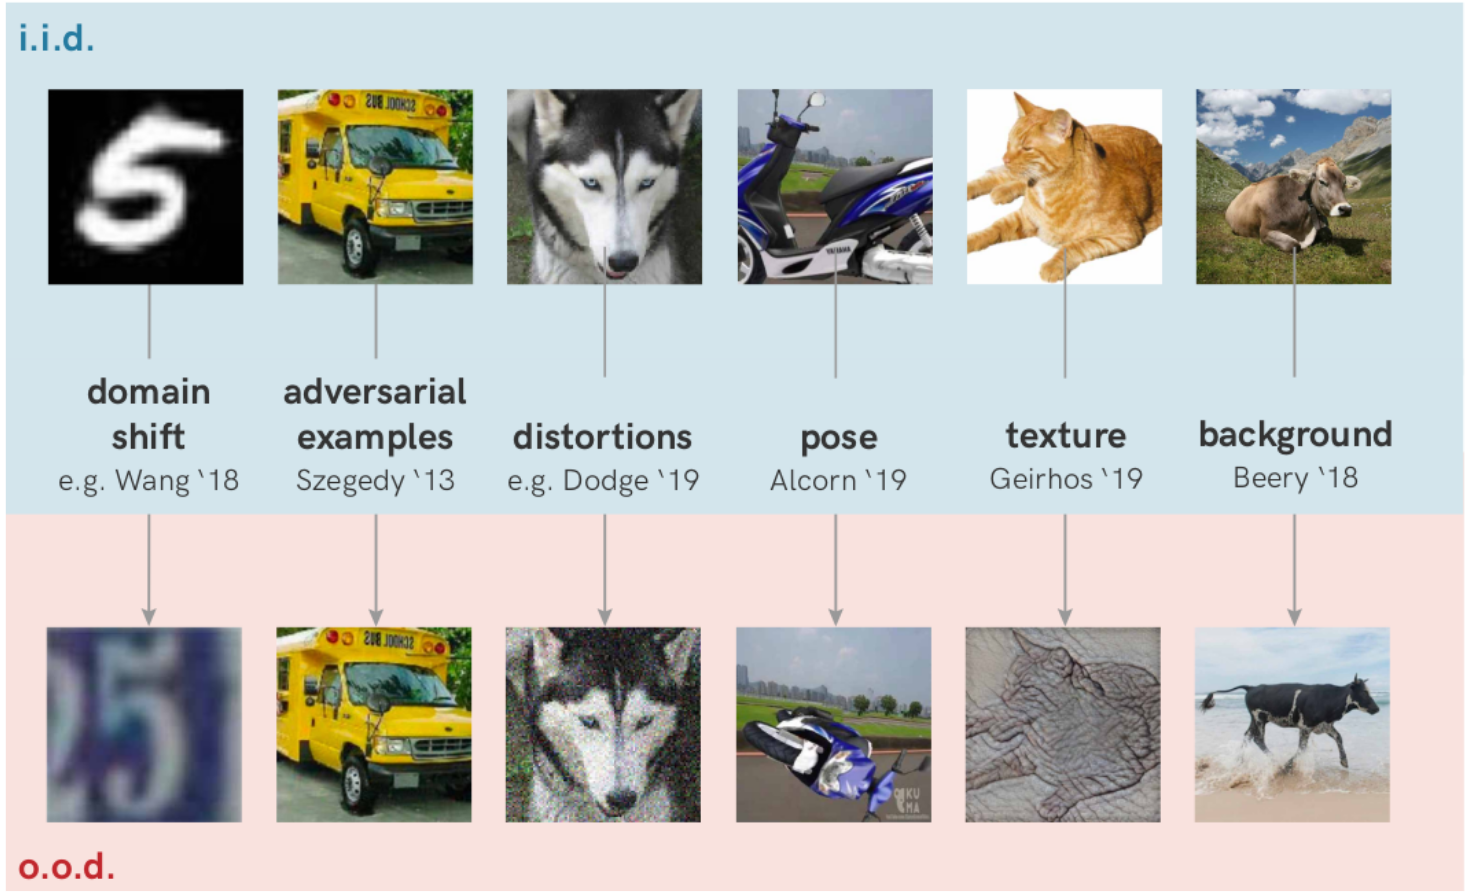
\includegraphics[width=0.9\textwidth]{shortcuts_00}
  \end{figure}

  \note{
    \begin{itemize}
      \item They learn shortcuts if we let them.
      \item Image from Shortcut Learning in Deep Neural Networks, Geirhos et al, Nature Machine Intelligence 2020
    \end{itemize}
  }
\end{frame}


\begin{frame}{Neural Networks are lazy}
  \begin{figure}
    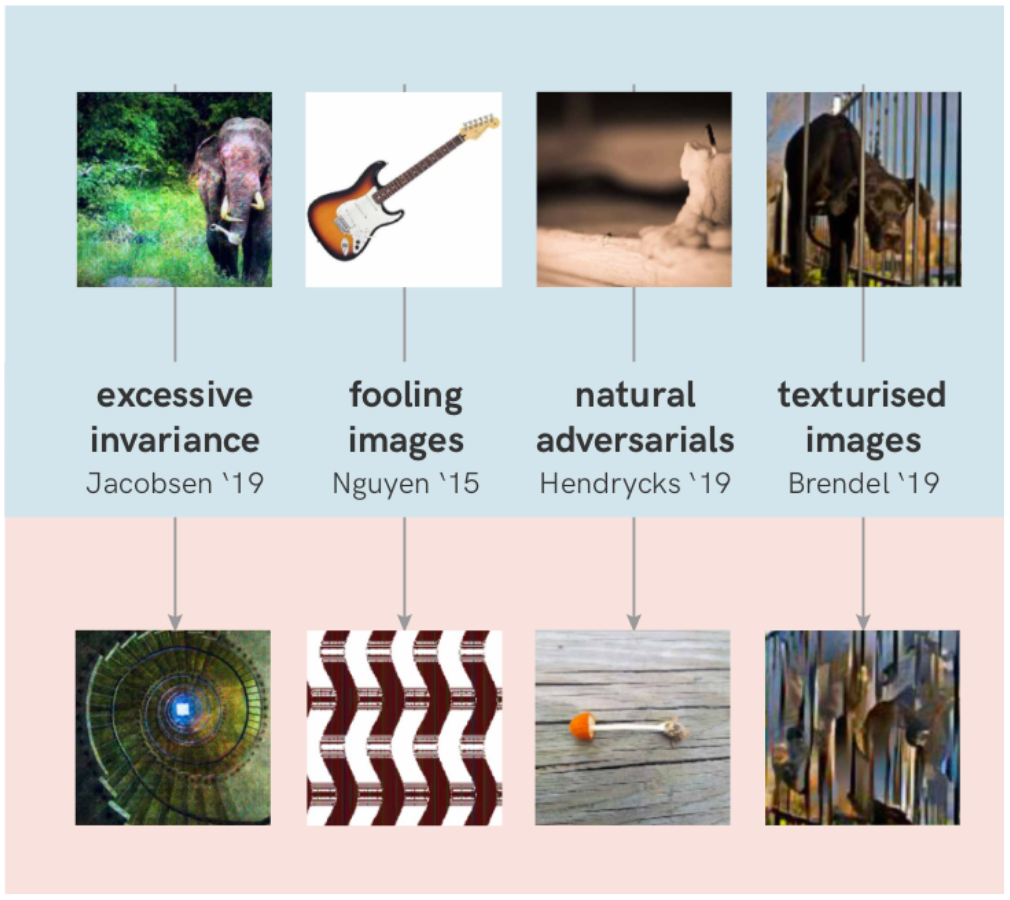
\includegraphics[width=0.6\textwidth]{shortcuts_01}
  \end{figure}

  \note{
    \begin{itemize}
      \item
      \item
      \item Image from Shortcut Learning in Deep Neural Networks, Geirhos et al, Nature Machine Intelligence 2020
    \end{itemize}
  }
\end{frame}


\begin{frame}{Investigate decisions: partial occlusion}
  \begin{figure}
    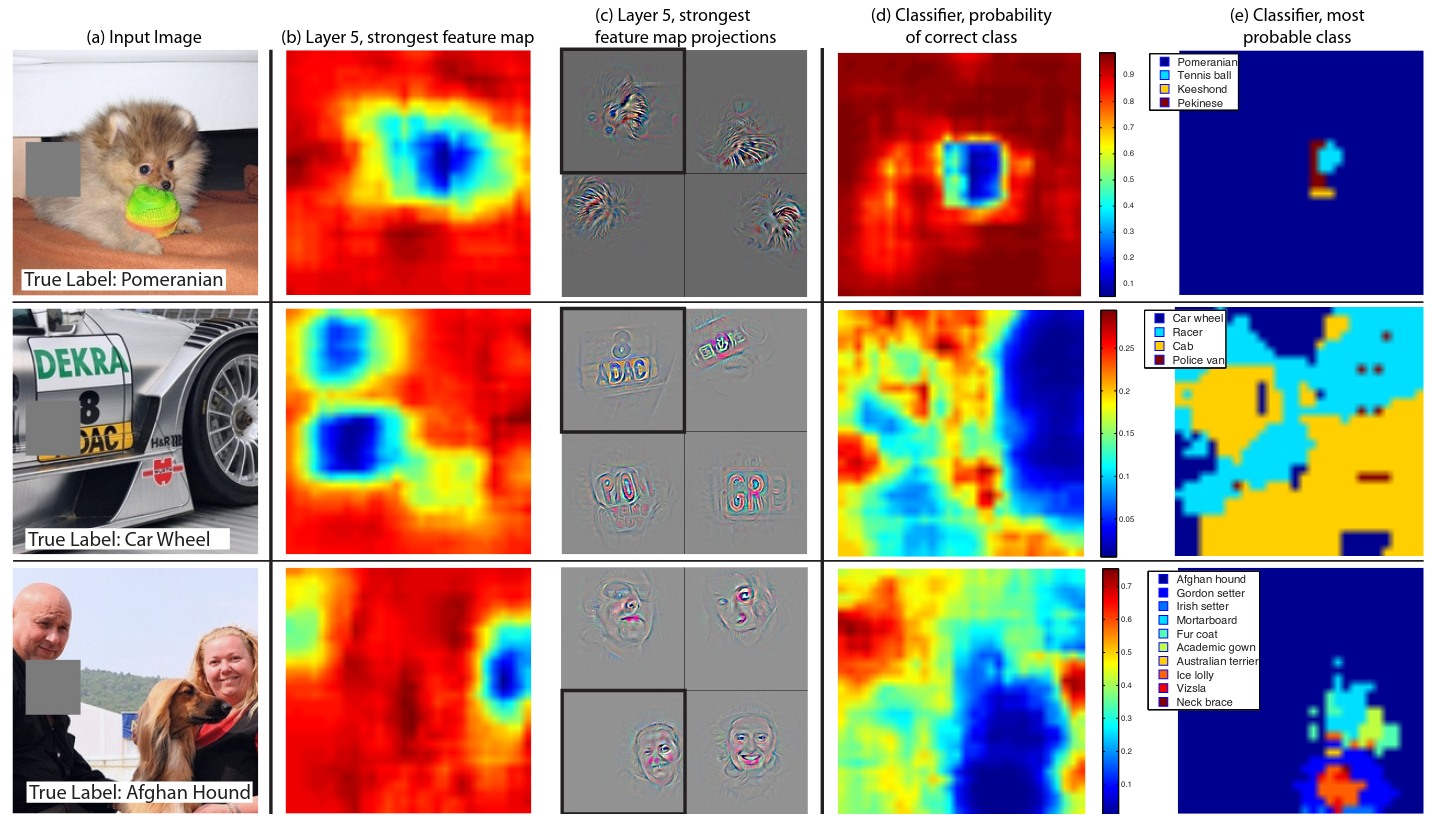
\includegraphics[width=0.9\textwidth]{occlusion}
  \end{figure}

  \note{
    \begin{itemize}
      \item An easy way for an visual sanity check is occluding parts of the image while watching the accuracy.
      \item Image from Visualizing and Understanding Convolutional Networks, Zeiler \& Fergus, ECCV 2014
    \end{itemize}
  }
\end{frame}


\begin{frame}{Investigate decisions: image gradient}
  \begin{figure}
    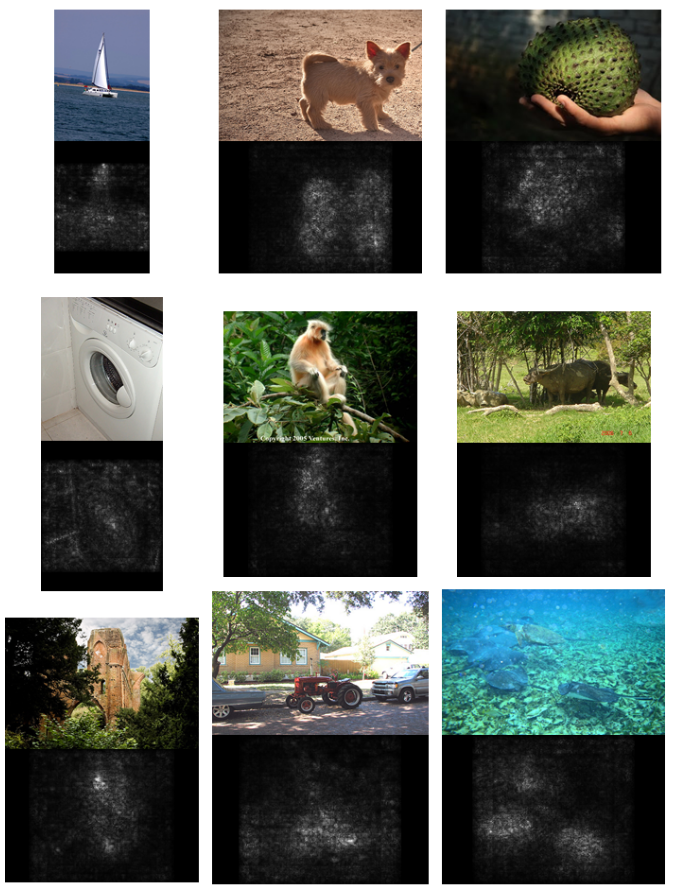
\includegraphics[width=0.4\textwidth]{image_backprop}
  \end{figure}

  \note{
    \begin{itemize}
      \item Looking at the pixel gradient of the network gives some insights too.
      \item Image from Deep Inside Convolutional Networks: Visualising Image Classification Models and Saliency Maps, Simonyan et al, 2013
    \end{itemize}
  }
\end{frame}


\begin{frame}{Investigate decisions: relevance propagation}
  \begin{figure}
    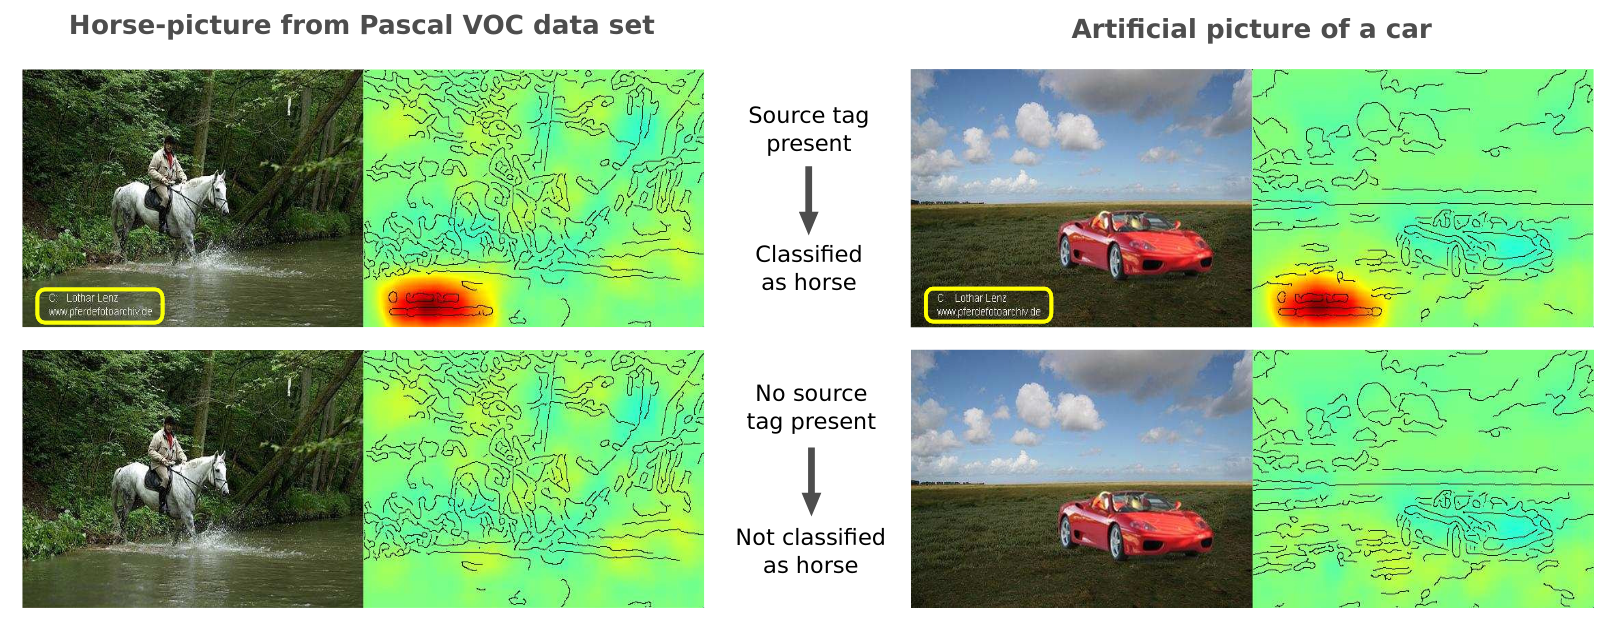
\includegraphics[width=0.9\textwidth]{relevance_propagation}
  \end{figure}

  \note{
    \begin{itemize}
      \item Explain the output, not the local variation.
      \item Image from Unmasking Clever Hans Predictors and Assessing What Machines Really Learn, Lapuschkin et al, Nature Communications 2019
    \end{itemize}
  }
\end{frame}


\end{document}
